\documentclass[10pt]{article}
\usepackage[utf8]{inputenc}
\usepackage[T1]{fontenc}
\usepackage{amsmath}
\usepackage{amsfonts}
\usepackage{amssymb}
\usepackage[version=4]{mhchem}
\usepackage{stmaryrd}
\usepackage{bbold}
\usepackage{caption}
\usepackage{hyperref}
\hypersetup{colorlinks=true, linkcolor=blue, filecolor=magenta, urlcolor=cyan,}
\urlstyle{same}
\usepackage{mathrsfs}
\usepackage{multirow}
\usepackage{graphicx}
\usepackage[export]{adjustbox}
\graphicspath{ {./images/} }

\title{Recovering or Testing Extended-Affine Equivalence }

\author{Anne Canteaut, Alain Couvreur, Léo Perrin}
\date{}


%New command to display footnote whose markers will always be hidden
\let\svthefootnote\thefootnote
\newcommand\blfootnotetext[1]{%
  \let\thefootnote\relax\footnote{#1}%
  \addtocounter{footnote}{-1}%
  \let\thefootnote\svthefootnote%
}

%Overriding the \footnotetext command to hide the marker if its value is `0`
\let\svfootnotetext\footnotetext
\renewcommand\footnotetext[2][?]{%
  \if\relax#1\relax%
    \ifnum\value{footnote}=0\blfootnotetext{#2}\else\svfootnotetext{#2}\fi%
  \else%
    \if?#1\ifnum\value{footnote}=0\blfootnotetext{#2}\else\svfootnotetext{#2}\fi%
    \else\svfootnotetext[#1]{#2}\fi%
  \fi
}

\begin{document}
\maketitle
\captionsetup{singlelinecheck=false}
May 17, 2022

\begin{abstract}
Extended Affine (EA) equivalence is the equivalence relation between two vectorial Boolean functions $F$ and $G$ such that there exist two affine permutations $A, B$, and an affine function $C$ satisfying $G=A \circ F \circ B+C$. While the problem has a simple formulation, it is very difficult in practice to test whether two functions are EA-equivalent. This problem has two variants: $E A$-partitioning deals with partitioning a set of functions into disjoint EA-equivalence classes, and $E A$-recovery is about recovering the tuple ( $A, B, C$ ) if it exists.\\
In this paper, we present a new algorithm that efficiently solves the EA-recovery problem for quadratic functions. Although its worst-case complexity occurs when dealing with APN functions, it supersedes, in terms of performance, all previously known algorithms for solving this problem for all quadratic functions and in any dimension, even in the case of APN functions. This approach is based on the Jacobian matrix of the functions, a tool whose study in this context can be of independent interest.\\
The best approach for EA-partitioning in practice mainly relies on class invariants. We provide an overview of the known invariants along with a new one based on the ortho-derivative. This new invariant is applicable to quadratic APN functions, a specific type of functions that is of great interest, and of which tens of thousands need to be sorted into distinct EA-classes. Our ortho-derivative-based invariant is very fast to compute, and it practically always distinguishes between EA-inequivalent quadratic APN functions.
\end{abstract}

\section*{1 Introduction}
Nonlinear vectorial Boolean functions (also known as Sboxes) are crucial building-blocks of most symmetric cryptosystems. For instance, their properties can be used to prove that a cryptographic primitive is safe from differential and linear cryptanalysis Nyb12. The search for vectorial Boolean functions that guarantee an optimal resistance to these attacks has then motivated a long line of research in the last 30 years. Indeed, establishing a list (as complete as possible) of optimal functions that could be used as Sboxes would be very helpful to designers of cryptographic primitives.

However, the huge number of vectorial Boolean functions from $\mathbb{F}_{2}^{n}$ into $\mathbb{F}_{2}^{m}$, even for small $n$ and $m$, makes an exhaustive search infeasible. In order to help in this task, the functions are then considered up to some equivalence relations which preserve the considered cryptographic properties. The most natural notions of equivalence are affine equivalence, and its generalization called extended affine equivalence, which are defined as follows.

Definition 1 ((Extended) Affine Equivalence). Two vectorial Boolean functions $F: \mathbb{F}_{2}^{n} \rightarrow \mathbb{F}_{2}^{m}$ and $G: \mathbb{F}_{2}^{n} \rightarrow \mathbb{F}_{2}^{m}$ are affine equivalent if $G=A \circ F \circ B$ for some affine permutations $A$ of $\mathbb{F}_{2}^{n}$ and $B$ of $\mathbb{F}_{2}^{m}$. They are extended affine equivalent ( $E A$-equivalent) if $G=A \circ F \circ B+C$ where $A$ and $B$ are as before and where $C: \mathbb{F}_{2}^{n} \rightarrow \mathbb{F}_{2}^{m}$ is an affine function.

Determining whether two functions $F, G: \mathbb{F}_{2}^{n} \rightarrow \mathbb{F}_{2}^{m}$ are affine or EA-equivalent is a problem that appears in several situations: when classifying vectorial Boolean functions, but also in cryptanalysis, where several types of attacks need to recover, if it exists, the transformation between two equivalent functions (see e.g. Din18 for details). This last situation then corresponds to the following problem, named $E A$-recovery, which is investigated in this paper.

Problem 1 (EA-recovery). Let $F$ and $G$ be two functions from $\mathbb{F}_{2}^{n}$ into $\mathbb{F}_{2}^{m}$. Find, if they exist, two affine permutations $A$ and $B$, and an affine function $C$ such that $G=A \circ F \circ B+C$.

But, in practice, the following variant of Problem 1 better captures some situations which occur in particular when classifying vectorial Boolean functions with good cryptographic properties.

Problem 2 (EA-partitioning). Let $\left\{F_{i}\right\}_{0 \leqslant i<\ell}$ be a set of $\ell$ functions from $\mathbb{F}_{2}^{n}$ into $\mathbb{F}_{2}^{m}$. Partition this set in such a way that any two functions in the same subset are $E A$-equivalent and no two functions belonging to distinct subsets are EA-equivalent.

Of course, EA-partitioning can be solved by applying an algorithm for EA-recovery to each pair $\left(F_{i}, F_{j}\right), i<j$. But, since we mainly focus on situations where the set of functions to be partitioned is large (for instance, around 20,000), examining all pairs of functions would be too computationally expensive. A situation where EA-partitioning of such a large set of functions is needed is related to one of the most prominent problems related to optimal cryptographic functions: the search for so-called Almost Perfect Nonlinear (APN) functions, which are the functions offering the best possible protection against differential cryptanalysis NK93 (see e.g. BN15 for a survey on APN functions). Most notably, the existence of APN bijective mappings in even dimensions $n>6$ is a long-standing open question known as the Big APN problem BDMW10. The only known APN permutation in even dimension was exhibited in 2009 by Dillon and his co-authors BDMW10 in dimension 6. It was derived from an APN quadratic non-bijective function by a more general notion of equivalence called CCZ-equivalence CCZ98. CCZ-equivalence expresses the fact that the graphs of the functions, i.e., the sets of the form $\left\{(x, F(x)): x \in \mathbb{F}_{2}^{n}\right\}$, are images of each other by an affine transformation. This notion is strictly more general than EA-equivalence BC10 but the two notions coincide for some particular cases including quadratic APN functions Yos11. Since Dillon et al.'s seminal work, a standard strategy, followed by many authors YWL14, CDP17, BL21, WTG13, to search for APN permutations in even dimension, consists in searching for quadratic APN non-bijective functions and in exploring their CCZ-equivalence class. To this end, it is important that the explored CCZ-equivalence classes be distinct. This equivalently means that they are generated from quadratic APN functions which are not EA-equivalent. Following this approach, around 20,000 of quadratic APN functions have been generated in YWL14 and [BL21] and it is necessary to check whether some of them belong to the same EA-equivalence class (or, equivalently, the same CCZ-class). The search for quadratic APN functions, which is motivated by the Big APN problem but may be of independent interest, is then the main relevant use-case for which we propose an efficient EA-partitioning procedure, which amounts to partitioning the functions into EA-classes based on their ortho-derivatives.

\subsection*{1.1 State of the Art: Affine-Equivalence Recovery in some Specific Cases}
A generic procedure for testing CCZ-, EA- and affine equivalence and, if it exists, for recovering the corresponding transformation, is derived from coding theory. Actually, the main cryptographic properties (e.g. the APN property) can be interpreted as conditions on some binary linear codes, as first shown in CCZ98. To this end, any function $F$ from $\mathbb{F}_{2}^{n}$ to $\mathbb{F}_{2}^{m}$ is associated to the linear\\
binary code $\mathcal{C}_{F}$ of length $2^{n}$ defined by the following $(n+m+1) \times 2^{n}$ generator matrix

$$
G_{F}=\left(\begin{array}{ccccc}
1 & \ldots & 1 & \ldots & 1 \\
0 & \ldots & x_{i} & \ldots & x_{2^{n}-1} \\
F(0) & \ldots & F\left(x_{i}\right) & \ldots & F\left(x_{2^{n}-1}\right)
\end{array}\right),
$$

where $\left\{0, x_{1}, \ldots, x_{2^{n}-1}\right\}$ denotes the set of all elements in $\mathbb{F}_{2}^{n}$ and each entry in the matrix is viewed as a binary column-vector. As observed in EP09, BDKM09, CCZ-equivalence then coincides with the usual notion of equivalence between two linear binary codes MS77, Page 39]. EAequivalence and affine equivalence also correspond to code equivalence, but for codes defined by a slightly different generator matrix (see Section 7 in EP09). A general technique for testing and recovering CCZ- and EA-equivalence then consists in applying an algorithm for testing the equivalence between two linear codes, e.g. Leo95, as proposed in EP09, Cal20. This algorithm is generic in the sense that it applies to any linear binary code, not only to codes associated to vectorial Boolean functions. But the downside is that it is expensive in terms of both time and memory. For instance, its implementation in SAGE [ $\mathrm{S}^{+} 19$ ] requires at least 40 seconds to check the CCZ-equivalence of two 8-bit functions, which is often prohibitively expensive since this verification must be done for many pairs of functions. For 9-bit functions, it may crash from lack of memory, though the machine on which we performed this test has 32 GB of RAM. While Magma [CFS14] might be faster, it is not as easily available (Magma is not free). More importantly, as noted in Kal21b, p. 20], the routine verifying CCZ-equivalence in Magma cannot be run for $n=12$ (even on a supercomputer with 500 GB of RAM). Even for $n \in\{9,10\}$, it sometimes requires several hours and may report wrong results.

However, since EA-recovery is a specific instance of the code equivalence problem, it might be possible a more efficient algorithm if we focus on codes of the form $\mathcal{C}_{F}$. But very few results are known even when $F$ belongs to some particular families of functions. Instead, algorithms for solving several particular cases, when $A, B$ or $C$ have a specific form, have been proposed based on other techniques, for instance in BK12 and ÖSY14. The case $C=0$ (corresponding to affine equivalence) has been solved when $F$ and $G$ are permutations in the sense that we have algorithms capable of finding $A$ and $B$ in this context BDBP03.

\subsection*{1.1.1 Guess-and-Determine}
The first algorithm for affine equivalence recovery was proposed in BDBP03. It is based on a subroutine which returns the "linear representative" of a permutation. Given a permutation $F$, it returns the two linear permutations $L_{0}$ and $L_{1}$ such that, among all the possible choices for $L_{0}, L_{1}$, the linear permutation $L_{1} \circ F \circ L_{0}$ is the smallest with respect to the lexicographic order. This algorithm is based on a guess-and-determine approach. Its authors estimated its time complexity to be $\mathrm{O}\left(n^{3} 2^{n}\right)$ if $F(0) \neq 0$ and $\mathrm{O}\left(n^{3} 2^{2 n}\right)$ otherwise.

We have implemented this algorithm and, in practice, the running time can be worse than this. Indeed, the complexity analysis assumes that a contradiction in the guess-and-determine procedure will occur after a small number of guesses. This is usually true but, in some cases, it may happen that all values for a variable need to be tested. In this case, the claimed complexity is multiplied by a factor $2^{n}$.

Using this algorithm, it is easy to recover $A$ and $B$ when they are linear. However, when they are affine, we also need to perform an exhaustive search for the constants $A(0)$ and $B(0)$. In this case, we generate two lists containing the linear representatives of $x \mapsto F(x \oplus a)$ and $x \mapsto b \oplus G(x)$. We then check if there is a match in these lists, i.e., an entry that belongs to both lists. Both the time and memory complexities in this case are multiplied by $2^{n}$. The overall time is then $\mathrm{O}\left(n^{3} 2^{2 n}\right)$ (if we assume that the complexity estimation of the authors of BDBP03 is correct).

This method works for all permutations. But its downsides are that its complexity is underestimated in some cases and that it does not apply to non-bijective mappings.

\subsection*{1.1.2 Rank Table}
In a more recent paper Din18, Dinur proposed a completely different approach based on socalled "rank tables". Paraphrasing the introduction of said paper, the main idea of the algorithm is to compute the rank tables of both $F$ and $G$ and then use these tables to recover the affine transformation $B$, assuming that $G=A \circ F \circ B$. The rank tables of $F$ and $G$ are obtained as follows. We derive from $F$ (resp. from $G$ ) several functions, each one defined by restricting its $2^{n}$ inputs to an affine subspace of dimension $n-1$. Each function derived in this way has an associated rank, corresponding to the rank of the matrix formed by the vectors representing the algebraic normal forms of its coordinates (see Section 2 for the definitions of the notions). We then assign to each possible $(n-1)$-dimensional subspace a corresponding rank. As there are $\left(2^{n+1}-2\right)$ possible affine subspaces, we obtain $\left(2^{n+1}-2\right)$ rank values for $F$ (resp. for $G$ ). These values are collected in the rank table of $F$ (resp. $G$ ), where a rank table entry $r$ stores the set of all affine subspaces to which a rank of $r$ has been assigned. We then look for matches in these two rank tables.

This approach is faster than the algorithm of Biryukov et al., as the computational time for affine equivalence recovery is $\mathrm{O}\left(n^{3} 2^{n}\right)$, i.e. it is $2^{n}$ times faster. Unlike the latter, the rank tablebased approach works even if the functions are not bijective; but it does require that their algebraic degree is high enough, i.e. at least $n-2$ Din18. We have used an implementation of this algorithm by its author and we have confirmed that it could very efficiently handle non-bijective functions of degree $n-1$. However, for functions of degree $n-2$, the rank tables of the test functions turn out to contain a single value. In such a situation the algorithm is not faster than an exhaustive search, and is therefore not relevant.

\subsection*{1.2 Our Results}
While the two previously mentioned algorithms are dedicated to affine equivalence recovery, i.e, to the case $C=0$, we present here the first efficient algorithm for $E A$-equivalence recovery in any dimension, when the involved functions $F$ and $G: \mathbb{F}_{2}^{n} \rightarrow \mathbb{F}_{2}^{m}$ are quadratic. Our algorithm works both on permutations and non-bijective functions. We prove that its complexity depends on the differential spectrum of the function and is estimated to be $\mathrm{O}\left(\max (n, m)^{\omega} 2^{n}+R^{s}\left(m^{2}+n^{2}\right)^{\omega}\right)$, where $\omega \simeq 2.37$ denotes the complexity exponent of matrix multiplication and $R$ is the number of vectors $v \in \mathbb{F}_{2}^{n} \backslash\{0\}$ at which the rank of the Jacobian matrix is the smallest possible. The last parameter $s$ is a number of guesses which, when $m=n$, can be chosen to be equal to 3 . Hence, the estimated complexity is $\mathrm{O}\left(n^{\omega} 2^{n}+R^{3} n^{2 \omega}\right)$ and it turns out that, for vectorial Boolean functions chosen at random, the quantity $R$ is frequently very small. On the other hand, the most difficult case corresponds to APN functions where the complexity is $\mathrm{O}\left(2^{2 n}\left(m^{2}+n^{2}\right)^{\omega}\right)$.

The second part of the paper details several tools for solving the $E A$-partitioning problem. Most notably, we propose some new and very efficient EA-invariants for quadratic APN functions, which is one of the most important instances of this problem. This technique is then used to partition the CCZ-classes of all the 6 -bit quadratic APN functions into EA-classes. Also, by applying this method to 8 -bit quadratic APN functions, we show that it is by far the most efficient one for solving Problem 2 in the case of quadratic APN functions.

It is worth noting that, as detailed in Table 1, only some problems related to EA-equivalence have been solved. Several simplified cases have been solved in BK12, ÖSY14, where some of the involved affine functions correspond to the identity or to the addition of a constant. In a very recent and concurrent work Kal20 (independent of ours) another EA-recovery algorithm\\
is presented by Kaleyski which is based on a new EA-invariant called $\Sigma^{k}$-multiplicities. This algorithm is efficient and is not restricted to quadratic functions but it applies to even dimensions only. Indeed, it has been observed that the underlying invariant does not provide any useful information in odd dimensions. Its complexity, while low enough in practice, is hard to estimate due to its reliance on backtracking. However, finding a general algorithm for EA-recovery, faster than generic techniques for recovering code equivalence, for functions of degree strictly greater than two and for any dimension, remains an open problem.

\begin{table}[h]
\begin{center}
\begin{tabular}{|l|l|l|}
\hline
Condition & Complexity & Reference \\
\hline
$C=0, m=n, F$ and $G$ bijective & O $\left(n^{3} 2^{2 n}\right)$ & BDBP03 \\
\hline
$C=0, \operatorname{deg}(F) \geqslant n-1$ & O $\left(n^{3} 2^{n}\right)$ & Din18 \\
\hline
$A(x)=x \oplus a, B(x)=x \oplus b$ & $\mathrm{O}\left(n 2^{n}\right)$ & BK12 \\
\hline
$A(x)=x, B(0)=0$ & O $\left(2^{n}\right)$ & ÖSY14 \\
\hline
$B(x)=x \oplus b$ & $\mathrm{O}\left(m 2^{3 n}\right)$ & BK12 \\
\hline
$\operatorname{deg}(F)=2$ & $\mathrm{O}\left(n^{2 \omega} 2^{2 n}\right)$ & Section 3.4 \\
\hline
$n$ even & - & Kal21a \\
\hline
\end{tabular}
\captionsetup{labelformat=empty}
\caption{Table 1: Algorithms solving the EA-recovery of $F: \mathbb{F}_{2}^{n} \rightarrow \mathbb{F}_{2}^{m}$ and $G=A \circ F \circ B+C$. See Section 4.1 for an overview of EA-partitioning.}
\end{center}
\end{table}

Organization of the Paper. We first recall the basic concepts and definitions needed in Section 2.\\
The rest of the paper successively presents our results that can efficiently tackle both Problems 1 and 2 in the case of quadratic functions. First, we show how to reduce EA-recovery to the resolution of a linear system using the Jacobian matrix. This approach is described in Section 3 .

Then, Section 4 first describes a general approach based on class invariants which can solve EA-partitioning (Problem 2), and lists all the CCZ- and EA-class invariants we are aware of from the literature. Then, in the case of quadratic APN functions, we introduce a new invariant based on ortho-derivatives. It is very discriminating, and can efficiently prove that more than 20,000 distinct quadratic APN functions of 8 variables fall into different CCZ-classes in only a few minutes on a regular desktop computer.

Our optimized implementations of all these invariants are available in the Sage package sboxu $\unlhd^{1}$

\section*{2 Preliminaries and Definitions}
We consider vectorial Boolean functions, that is functions from the vector space $\mathbb{F}_{2}^{n}$ to the vector space $\mathbb{F}_{2}^{m}$ for some non-zero $m$ and $n$. When $m=1$, such functions are called Boolean functions. Any vectorial Boolean function can be represented in different ways. For instance, it can be seen as a sequence of $m$ Boolean functions from $\mathbb{F}_{2}^{n}$ to $\mathbb{F}_{2}$, called its coordinates. Each of these $m$ coordinates can be uniquely written as a multivariate polynomial in $\mathbb{F}_{2}\left[x_{1}, \ldots, x_{n}\right] /\left(x_{1}^{2}+x_{1}, \ldots, x_{n}^{2}+x_{n}\right)$, called its Algebraic Normal Form (ANF). A vectorial Boolean function can also be represented by its truth table (aka look-up table), which is the array composed of all its output values. The following notions will be extensively used throughout the paper.

\footnotetext{${ }^{1}$ sboxU is available for download at \href{https://github.com/lpp-crypto/sboxU}{https://github.com/lpp-crypto/sboxU}
}Differential Properties. The resilience of a function to differential attacks BS91 is expressed by simple properties of its derivatives.

Definition 2 (Derivative). Let $F$ be a function from $\mathbb{F}_{2}^{n}$ into $\mathbb{F}_{2}^{m}$. The derivative of $F$ with respect to $a \in \mathbb{F}_{2}^{n}$ is the function from $\mathbb{F}_{2}^{n}$ into $\mathbb{F}_{2}^{m}$ defined by

$$
\Delta_{a} F: x \in \mathbb{F}_{2}^{n} \mapsto F(x+a)+F(x) .
$$

In practice, the properties of the derivatives are analyzed through the multiset introduced below which corresponds to the entries of its difference distribution table (DDT).

Definition 3 (DDT, differential spectrum). Let $F$ be a function from $\mathbb{F}_{2}^{n}$ into $\mathbb{F}_{2}^{m}$. The DDT of $F$ is the $2^{n} \times 2^{m}$ array consisting of all elements

$$
\delta_{F}(a, b):=\#\left\{x \in \mathbb{F}_{2}^{n}: F(x+a)+F(x)=b\right\}, \text { for }(a, b) \in \mathbb{F}_{2}^{n} \times \mathbb{F}_{2}^{m} .
$$

The differential uniformity of $F$ Nyb94 is defined as

$$
\delta(F):=\max _{a \in \mathbb{F}_{2}^{n} \backslash\{0\}, b \in \mathbb{F}_{2}^{m}} \delta_{F}(a, b),
$$

and the differential spectrum of $F$ is the multiset

$$
\left[\delta_{F}(a, b), a \in \mathbb{F}_{2}^{n}, a \neq 0, b \in \mathbb{F}_{2}^{m}\right] .
$$

Obviously, $\delta(F) \geqslant 2^{n-m}$ and the functions for which equality holds are called Perfect Nonlinear or bent. Such functions exist only when $n$ is even and $m \leqslant n / 2$ Nyb91. When $m \geqslant n$, the differential uniformity satisfies $\delta(F) \geqslant 2$, and the functions for which equality holds are called Almost Perfect Nonlinear (APN) functions.

Walsh Transform. Similarly, the resistance of a function to linear attacks Mat94 is evaluated through its Linear approximation table (LAT), whose entries are given by the Walsh transform.

Definition 4 (Walsh transform). Let $F$ be a function from $\mathbb{F}_{2}^{n}$ into $\mathbb{F}_{2}^{m}$. Its Walsh transform at $(a, b) \in \mathbb{F}_{2}^{n} \times \mathbb{F}_{2}^{m}$ is the integer defined by

$$
\mathcal{W}_{F}(a, b):=\sum_{x \in \mathbb{F}_{2}^{n}}(-1)^{a \cdot x+b \cdot F(x)}
$$

where $y \cdot z$ denotes the canonical inner product on $\mathbb{F}_{2}^{n}$, i.e. $y \cdot z:=\sum_{i=1}^{n} y_{i} z_{i}$ where $y=\left(y_{1}, \ldots, y_{n}\right)$ and $z=\left(z_{1}, \ldots, z_{n}\right)$. The Walsh spectrum of $F$ is then the multiset

$$
\left[\mathcal{W}_{F}(a, b): a \in \mathbb{F}_{2}^{n}, b \in \mathbb{F}_{2}^{m}\right] .
$$

Degree. The degree of a vectorial Boolean function is defined as follows.\\
Definition 5 (Degree). Let $F$ be a function from $\mathbb{F}_{2}^{n}$ into $\mathbb{F}_{2}^{m}$. The degree of $F$ is the maximal degree of the algebraic normal forms of its coordinates.

The functions of degree less than or equal to 1 are said to be affine. Quadratic functions, i.e. functions of degree 2 , will also play an important role in this paper.

CCZ-Equivalence. While this paper focuses on EA-equivalence, there exists a more general notion of equivalence between vectorial Boolean functions defined by Carlet, Charpin and Zinoviev CCZ98 and called CCZ-equivalence. This notion will be widely used in Section 4.

Definition 6. Two functions $F: \mathbb{F}_{2}^{n} \rightarrow \mathbb{F}_{2}^{m}$ and $G: \mathbb{F}_{2}^{n} \rightarrow \mathbb{F}_{2}^{m}$ are $C C Z$-equivalent if there exists an affine permutation $\mathcal{A}$ of $\mathbb{F}_{2}^{n} \times \mathbb{F}_{2}^{m}$ such that

$$
\mathcal{A}\left(\left\{(x, F(x)): x \in \mathbb{F}_{2}^{n}\right\}\right)=\left\{(x, G(x)): x \in \mathbb{F}_{2}^{n}\right\} .
$$

Two functions which are EA-equivalent are also CCZ-equivalent (see Car21, Page 29] for a proof), but the converse does not hold BCP06.

In general, given a function $F: \mathbb{F}_{2}^{n} \rightarrow \mathbb{F}_{2}^{m}$ and an affine permutation $\mathcal{A}$ of $\mathbb{F}_{2}^{n} \times \mathbb{F}_{2}^{m}$,

$$
\mathcal{A}\left(\left\{(x, F(x)): x \in \mathbb{F}_{2}^{n}\right\}\right)
$$

does not correspond to the graph of a function, i.e. to a set of the form $\left\{(x, G(x)): x \in \mathbb{F}_{2}^{n}\right\}$ for some function $G$ from $\mathbb{F}_{2}^{n}$ to $\mathbb{F}_{2}^{m}$. Indeed, for $G$ to be well-defined, it is necessary that the first $n$ coordinates of $x \mapsto \mathcal{A}(x, F(x))$ permute $\mathbb{F}_{2}^{n}$. As a consequence, only a few permutations $\mathcal{A}$ yield valid functions $G$. The following definition captures this intuition.

Definition 7 (Admissible affine permutations). Let $F$ be a function from $\mathbb{F}_{2}^{n}$ to $\mathbb{F}_{2}^{m}$. We say that the affine permutation $\mathcal{A}$ of $\mathbb{F}_{2}^{n} \times \mathbb{F}_{2}^{m}$ is admissible for $F$ if

$$
\mathcal{A}\left(\left\{(x, F(x)), x \in \mathbb{F}_{2}^{n}\right\}\right)
$$

is a graph of a function.

\section*{3 Recovering EA-equivalence for Quadratic Functions}
\subsection*{3.1 The Jacobian Matrix}
Notation 8. In the sequel, the canonical basis of $\mathbb{F}_{2}^{n}$ is denoted by $\left(e_{1}, \ldots, e_{n}\right)$.\\
Definition 9. Let $F$ be a function from $\mathbb{F}_{2}^{n}$ into $\mathbb{F}_{2}^{m}$. The Jacobian of $F$ at $x \in \mathbb{F}_{2}^{n}$ is the matrix with polynomial entries defined by

\[
\operatorname{Jac} F(x):=\left(\begin{array}{ccc}
\Delta_{e_{1}} F_{1}(x) & \cdots & \Delta_{e_{n}} F_{1}(x)  \tag{1}\\
\vdots & \ddots & \vdots \\
\Delta_{e_{1}} F_{m}(x) & \cdots & \Delta_{e_{n}} F_{m}(x)
\end{array}\right)
\]

On the other hand, given an $m$-tuple of polynomials $P=\left(P_{1}, \ldots, P_{m}\right) \in \mathbb{F}_{2}\left[X_{1}, \ldots, X_{n}\right]^{m}$, we define the Jacobian matrix of $P$ as

$$
\mathscr{J} P(x):=\left(\begin{array}{ccc}
\frac{\partial P_{1}}{\partial x_{1}} & \cdots & \frac{\partial P_{1}}{\partial x_{n}} \\
\vdots & & \vdots \\
\frac{\partial P_{m}}{\partial x_{1}} & \cdots & \frac{\partial P_{m}}{\partial x_{n}}
\end{array}\right) \in \mathbb{F}_{2}\left[X_{1}, \ldots, X_{n}\right]^{m \times n},
$$

where $\frac{\partial P_{i}}{\partial x_{j}}$ denotes the partial derivative of $P_{i}$ with respect to $x_{j}$.

Remark 10. The two notions are strongly related to each other. In particular, for a vectorial Boolean function $F: \mathbb{F}_{2}^{n} \rightarrow \mathbb{F}_{2}^{n}$, denote by $P_{F}^{\mathrm{ANF}} \in \mathbb{F}_{2}\left[X_{1}, \ldots, X_{n}\right]^{m}$ the polynomial representation of $F$ in algebraic normal form, then

$$
\operatorname{Jac} F(x)=\mathscr{J} P_{F}^{\mathrm{ANF}}(x) .
$$

This equality can be easily checked on monomials and then extended by linearity.\\
Note however the importance of being in algebraic normal form: for instance in one variable, if $P(x)=x^{2}$, then $\frac{\partial P}{\partial x}=0$, while the algebraic normal form of $P$ is $x$ whose derivative is 1 .

\subsection*{3.2 The Jacobian Matrices of EA-equivalent Functions}
Assume that $G=A \circ F \circ B+C$, for some affine permutations $A$ and $B$ and an affine function $C$ defined as

$$
\forall x \in \mathbb{F}_{2}^{n}, \quad A(x)=A_{0} x+a, \quad B(x)=B_{0} x+b, \quad \text { and } \quad C(x)=C_{0} x+c,
$$

where $A_{0}, B_{0}$ are non-singular matrices in $\mathbb{F}_{2}^{n \times n}$ and $\mathbb{F}_{2}^{m \times m}$ respectively, $C_{0}$ is a matrix in $\mathbb{F}_{2}^{n \times m}$, and $a, c \in \mathbb{F}_{2}^{m}$ and $b \in \mathbb{F}_{2}^{n}$. Note that, after replacing $a$ by $a+c$, one can assume that $c=0$ and hence that $C$ is linear. We always do so in the sequel.

Denote by $P_{F}$ some polynomial representation of $F$ (which is not necessarily its ANF). Then consider the polynomial representation $P_{G}$ of $G$ defined by

$$
P_{G}:=A \circ P_{F} \circ B+C .
$$

Then, considering Jacobian matrices, one can apply the well-known chain rule formula for functions of several variables, i.e. the formula for the Jacobian of compositions of functions, namely:


\begin{equation*}
\mathscr{J} P_{G}(x)=A_{0} \cdot \mathscr{J} P_{F}(B(x)) \cdot B_{0}+C_{0} . \tag{2}
\end{equation*}


Indeed, the Jacobians of $A, B$ and $C$ are $A_{0}, B_{0}$ and $C_{0}$, respectively. Unfortunately, this chain rule formula does not extend to Jacobians of Boolean functions because, as already observed in Remark 10, the operations of derivation and of reduction to the algebraic normal form do not commute. To clarify this issue, let us consider an elementary example.\\
Example 11. Let $P_{F}\left(x_{1}, x_{2}\right)=x_{1} x_{2}$ be a polynomial representing a function $F: \mathbb{F}_{2}^{2} \rightarrow \mathbb{F}_{2}$. Consider the linear map $B:\left(x_{1}, x_{2}\right) \mapsto\left(x_{1}+x_{2}, x_{2}\right)$. Set $P_{G}:=P_{F} \circ B=x_{1} x_{2}+x_{2}^{2}$. This polynomial represents a function $G$ whose algebraic normal form is $P_{G}^{\mathrm{ANF}}=x_{1} x_{2}+x_{2}$. Now, the Jacobian matrices of $F$ and $G$ are

$$
\operatorname{Jac} F(x)=\left(\begin{array}{ll}
x_{2} & x_{1}
\end{array}\right) \quad \text { and } \quad \operatorname{Jac} G(x)=\left(\begin{array}{ll}
x_{2} & x_{1}+1
\end{array}\right)
$$

and

$$
\operatorname{Jac} F(B(x))\left(\begin{array}{ll}
1 & 1 \\
0 & 1
\end{array}\right)=\left(\begin{array}{ll}
x_{2} & x_{1}+x_{2}
\end{array}\right)\left(\begin{array}{ll}
1 & 1 \\
0 & 1
\end{array}\right)=\left(\begin{array}{ll}
x_{2} & x_{1}
\end{array}\right),
$$

which differs from $\operatorname{Jac} G(x)$. On the other hand, if we consider polynomials instead of Boolean functions, we have

$$
\mathscr{J} P_{F}(B(x))\left(\begin{array}{ll}
1 & 1 \\
0 & 1
\end{array}\right)=\left(\begin{array}{ll}
x_{2} & x_{1}
\end{array}\right)=\mathscr{J} P_{G}(x) .
$$

While we observed that the chain rule formula in several variables is false in general for Boolean functions, we prove in the sequel that, in the context of quadratic functions, it is possible to get a very similar formula using the so-called linear part of the Jacobian. This will be the central idea of our algorithm.

\subsection*{3.3 The Jacobian Matrix of a Quadratic Function}
From now on, we assume that $F$ is quadratic, i.e. its algebraic normal form has degree 2. In this case, the entries of the associated Jacobian matrix, in the sense of Definition 9, are polynomials of degree 1 , and we will focus on their homogeneous parts.

Definition 12. Let $F: \mathbb{F}_{2}^{n} \rightarrow \mathbb{F}_{2}^{m}$ be a quadratic function. We denote by $\operatorname{Jac}_{\operatorname{lin}} F(x)$ the linear part of $\operatorname{Jac} F(x)$, i.e. the matrix whose entries are the homogeneous parts of degree 1 of the entries of $\operatorname{Jac} F(x)$ :

$$
\forall x \in \mathbb{F}_{2}^{n}, \quad \operatorname{Jac} F(x)=\operatorname{Jac}_{\operatorname{lin}} F(x)+\operatorname{Jac} F(0)
$$

Equivalently, $\operatorname{Jac}_{\text {lin }} F(x)=\left(J_{i, j}(x)\right)_{i, j}$ with


\begin{equation*}
J_{i, j}(x)=\Delta_{e_{j}} F_{i}(x)+\Delta_{e_{j}} F_{i}(0), \forall x \in \mathbb{F}_{2}^{n}, 1 \leqslant i \leqslant m, 1 \leqslant j \leqslant n, \tag{3}
\end{equation*}


where ( $e_{1}, \ldots, e_{n}$ ) denotes the canonical basis of $\mathbb{F}_{2}^{n}$ (Notation 8).\\
It is worth noting that the linear part of the Jacobian of a quadratic function corresponds to the coefficients of the quadratic monomials in the algebraic normal forms of the coordinates of $F$. Equivalently, $\operatorname{Jac}_{\text {lin }} F(x)$ is the Jacobian of the degree- 2 homogeneous part of the algebraic normal form of $F$ as explained by the following statement.

Proposition 13. Let $F: \mathbb{F}_{2}^{n} \rightarrow \mathbb{F}_{2}^{m}$ be a quadratic function. Let

$$
F_{i}\left(x_{1}, \ldots, x_{n}\right)=\sum_{k<\ell} Q_{k, \ell}^{i} x_{k} x_{\ell}+\sum_{k=1}^{n} c_{k}^{i} x_{k}+\varepsilon^{i}
$$

be the algebraic normal form of the $i$-th coordinate of $F, 1 \leqslant i \leqslant m$, where all coefficients $Q_{k, \ell}^{i}, c_{k}^{i}, \varepsilon^{i}$ lie in $\mathbb{F}_{2}$ and $Q_{k, \ell}^{i}=0$ when $k \geqslant \ell$. Then, the entries $J_{i, j}(x)$ of $\operatorname{Jac}_{\text {lin }} F(x)$ are

$$
J_{i, j}(x)=\sum_{k=1}^{n}\left(Q_{k, j}^{i}+Q_{j, k}^{i}\right) x_{k}, 1 \leqslant i \leqslant m, 1 \leqslant j \leqslant n .
$$

Proof. For any $i$ and $j, 1 \leqslant i \leqslant m$ and $1 \leqslant j \leqslant n$, we have

$$
\Delta_{e_{j}} F_{i}(x)=\sum_{k<j} Q_{k, j}^{i} x_{k}+\sum_{k>j} Q_{j, k}^{i} x_{k}+c_{j}^{i}
$$

We then deduce from (3) that

$$
J_{i, j}(x)=\Delta_{e_{j}} F_{i}(x)+\Delta_{e_{j}} F_{i}(0)=\sum_{k=1}^{n}\left(Q_{k, j}^{i}+Q_{j, k}^{i}\right) x_{k} .
$$

The linear part of the Jacobian of a quadratic function is a useful mathematical object since the values of all derivatives of the function can be derived from this matrix, as shown in the following proposition.

Proposition 14. Let $F: \mathbb{F}_{2}^{n} \rightarrow \mathbb{F}_{2}^{m}$ be a quadratic function and let

$$
\operatorname{Jac}_{\operatorname{lin}} F(x)=\left(J_{i, j}(x)\right)_{1 \leqslant i \leqslant m, 1 \leqslant j \leqslant n}
$$

be the linear part of its Jacobian. Then, for any $a=\left(a_{1}, \ldots, a_{n}\right) \in \mathbb{F}_{2}^{n}$, any $i \in\{1, \ldots, m\}$ and any $x \in \mathbb{F}_{2}^{n}$, we have:

$$
\Delta_{a} F_{i}(x)+\Delta_{a} F_{i}(0)=\sum_{j=1}^{n} a_{j} J_{i, j}(x) .
$$

Hence, for any $a \in \mathbb{F}_{2}^{n}$ and any $x \in \mathbb{F}_{2}^{n}$, we have:

$$
\Delta_{a} F(x)+\Delta_{a} F(0)=\Delta_{x} \Delta_{a} F(0)=\operatorname{Jac}_{l i n} F(x) \cdot a=\operatorname{Jac}_{l i n} F(a) \cdot x .
$$

Proof. Let us first observe that, for any $a, x \in \mathbb{F}_{2}^{n}$,

$$
\Delta_{a} F(x)+\Delta_{a} F(0)=F(x+a)+F(x)+F(a)+F(0)=\Delta_{x} \Delta_{a} F(0)
$$

and hence

$$
\Delta_{a} F(x)+\Delta_{a} F(0)=\Delta_{x} F(a)+\Delta_{x} F(0)
$$

Let $S=\left\{i: a_{i}=1,1 \leqslant i \leqslant n\right\}$. Then,

$$
\begin{aligned}
\sum_{j=1}^{n} a_{j} J_{i, j}(x) & =\sum_{j \in S}\left(\Delta_{e_{j}} F_{i}(x)+\Delta_{e_{j}} F_{i}(0)\right) \\
& =\sum_{j \in S}\left(\Delta_{x} F_{i}\left(e_{j}\right)+\Delta_{x} F_{i}(0)\right) \\
& =\Delta_{x} F_{i}\left(\sum_{j \in S} e_{j}\right)+\Delta_{x} F_{i}(0) \\
& =\Delta_{x} F_{i}(a)+\Delta_{x} F_{i}(0) \\
& =\Delta_{a} F_{i}(x)+\Delta_{a} F_{i}(x) .
\end{aligned}
$$

The following corollary is another direct consequence of Proposition 14.\\
Corollary 15. Let $F: \mathbb{F}_{2}^{n} \rightarrow \mathbb{F}_{2}^{m}$ be a quadratic function. Then, for any a $\in \mathbb{F}_{2}^{n}$, we have

$$
\mathrm{Jac}_{\operatorname{lin}} F(a) \cdot a=0
$$

Using Proposition 14, we can exhibit the relation between the linear parts of the Jacobians of two EA-equivalent quadratic functions. This relation is very close to the chain rule formula in differential calculus. In addition it will be of particular interest for recovering the triple of functions ( $A, B, C$ ) such that $G=A \circ F \circ B+C$ because it does not involve $C$.\\
Proposition 16. Let $F$ and $G$ be two $E A$-equivalent quadratic functions from $\mathbb{F}_{2}^{n}$ into $\mathbb{F}_{2}^{m}$ with $G=A \circ F \circ B+C$ for some affine permutations $A$ and $B$, and some affine function $C$. Then,


\begin{equation*}
\forall x \in \mathbb{F}_{2}^{n}, \quad \mathrm{Jac}_{\text {lin }} G(x)=A_{0} \cdot \mathrm{Jac}_{\text {lin }} F(B(x)) \cdot B_{0} \tag{4}
\end{equation*}


where $A_{0}$ and $B_{0}$ denote the matrices corresponding to the linear parts of $A$ and $B$.\\
Proof. Let $A_{0}, B_{0}$ and $C_{0}$ denote the matrices corresponding to the linear parts of $A, B$ and $C$. Then, for any $a$ and $x$ in $\mathbb{F}_{2}^{n}$,

$$
\begin{aligned}
\Delta_{a} G(x)+\Delta_{a} G(0) & =\Delta_{a}(A \circ F \circ B)(x)+\Delta_{a}(A \circ F \circ B)(0) \\
& =A_{0}\left(\Delta_{a}(F \circ B)(x)+\Delta_{a}(F \circ B)(0)\right) \\
& =A_{0}\left(\Delta_{B_{0}(a)} F(B(x))+\Delta_{B_{0}(a)} F(B(0))\right) .
\end{aligned}
$$

It follows that Column $j$ of $\mathrm{Jac}_{\text {lin }} G(x)$ is equal to

$$
A_{0}\left[\Delta_{B_{0}\left(e_{j}\right)} F(B(x))+\Delta_{B_{0}\left(e_{j}\right)} F(B(0))\right]=A_{0} \cdot \mathrm{Jac}_{\operatorname{lin}} F(B(x)) \cdot B_{0}\left(e_{j}\right)
$$

where the equality is derived from Proposition 14. Therefore, Column $j$ of $\mathrm{Jac}_{\text {lin }} G(x)$ is equal to Column $j$ of $A_{0} \cdot \mathrm{Jac}_{\text {lin }} F(B(x)) \cdot B_{0}$.

It is worth noting that, when $m=n$, the linear part of the Jacobian, for quadratic functions defined by a homogeneous polynomia ${ }^{2}$ in $\mathbb{F}_{2^{n}}[X]$, is related to a special class of symmetric matrices over $\mathbb{F}_{2^{n}}$ called QAM and introduced in [YWL14]. This notion of QAM arises by exhibiting a one-to-one correspondence between the functions over $\mathbb{F}_{2}^{n}$ associated to a quadratic homogeneous univariate polynomial (i.e., with quadratic terms only) and symmetric matrices over $\mathbb{F}_{2^{n}}$ with diagonal elements equal to zero YWL14. This correspondence is detailed in the following definition.

Definition 17 (YWL14). Let $\mathcal{B}=\left(\alpha_{1}, \alpha_{2}, \ldots, \alpha_{n}\right)$ be a basis of $\mathbb{F}_{2^{n}}$ over $\mathbb{F}_{2}$ and $\varphi$ be the function from $\mathbb{F}_{2}^{n}$ to $\mathbb{F}_{2^{n}}$ defined by $\varphi\left(x_{1}, \ldots, x_{n}\right)=\sum_{i=1}^{n} x_{i} \alpha_{i}$. Let $P(X)=\sum_{k<\ell} q_{k, \ell} X^{2^{k-1}+2^{\ell-1}}$ be a quadratic homogeneous polynomial in $\mathbb{F}_{2^{n}}[X]$, and $F: \mathbb{F}_{2}^{n} \rightarrow \mathbb{F}_{2}^{n}$ be the quadratic vectorial Boolean function corresponding to $P$, i.e., defined by

$$
F(x)=\varphi^{-1} \circ P \circ \varphi(x), \quad \text { for all } x \in \mathbb{F}_{2}^{n}
$$

Then the matrix associated with $F$ with respect to $\mathcal{B}$ is

$$
H=M^{T} C_{P} M
$$

where $C_{P}$ is the $n \times n$ symmetric matrix over $\mathbb{F}_{2^{n}}$ defined by $\left(C_{P}\right)_{k, \ell}=\left(C_{P}\right)_{\ell, k}=q_{k, \ell}$ for all $1 \leqslant k<\ell \leqslant n,\left(C_{P}\right)_{k, k}=0$, and $M$ is the Moore matrix associated to $\mathcal{B}$, i.e., $M_{i, j}=\alpha_{j}^{2^{i-1}}$.

The advantage of this construction is that, when a function corresponds to a quadratic homogeneous univariate polynomial, being APN can be characterized by some algebraic properties of the associated matrix YWL14. We now show that the matrix $H=M^{T} C_{P} M$ is related to the linear part of the Jacobian of $F$.

Proposition 18. Let $F$ be a function from $\mathbb{F}_{2}^{n}$ to $\mathbb{F}_{2}^{n}$ corresponding to a quadratic homogeneous univariate polynomial for some basis $\mathcal{B}=\left(\alpha_{1}, \alpha_{2}, \ldots, \alpha_{n}\right)$, and let $H$ be the matrix associated with $F$ with respect to $\mathcal{B}$ in the sense of Definition 17. Then, for all $x \in \mathbb{F}_{2}^{n}$,

$$
\left(\alpha_{1}, \ldots, \alpha_{n}\right) \cdot \operatorname{Jac}_{l i n} F(x)=\left(x_{1}, \ldots, x_{n}\right) \cdot H
$$

Proof. Let $P$ be the homogeneous univariate polynomial associated to $F$ by $P=\varphi \circ F \circ \varphi^{-1}$, where $\varphi\left(x_{1}, \ldots, x_{n}\right)=\sum_{i=1}^{n} x_{i} \alpha_{i}$. Theorem 1 in YWL14 shows that, for any $j, 1 \leqslant j \leqslant n$, and any $X \in \mathbb{F}_{2^{n}}$,

$$
P\left(X+\alpha_{j}\right)+P(X)+P\left(\alpha_{j}\right)=\varphi(X) \cdot H_{j}
$$

where $H_{j}$ denotes Column $j$ of $H$. It follows that, for any $x \in \mathbb{F}_{2}^{n}$,

$$
(P \circ \varphi)\left(x+e_{j}\right)+P \circ \varphi(x)+P \circ \varphi\left(e_{j}\right)=x H_{j}
$$

or equivalently

$$
\varphi\left(F\left(x+e_{j}\right)+F(x)+F\left(e_{j}\right)\right)=x H_{j}
$$

\footnotetext{${ }^{2}$ Obviously, any quadratic function is EA-equivalent to a function corresponding to a univariate homogeneous polynomial of degree 2 .
}
which means that
$$
\sum_{i=1}^{n} \alpha_{i}\left[\operatorname{Jac}_{\operatorname{lin}} F(x)\right]_{i, j}=x H_{j}
$$

In other words, $\mathrm{Jac}_{\text {lin }} F(x)$ is three-dimensional in nature: when $m=n$, it is an $n \times n$ matrix whose entries are $n$-variable linear functions, represented by $n$ binary coefficients. The previous proposition shows that the matrix $H$ defined in YWL14 is another way to represent the same $2^{3 n}$ binary values, with a 2 -dimensional structure by using $\mathbb{F}_{2^{n}}$ as a coefficient field. Characterizing the fact that $F$ is APN from the properties of $H$ can then be reformulated in terms of Jacobians as we will prove in Section 3.4.2. However, our result applies also to functions from $\mathbb{F}_{2}^{n}$ to $\mathbb{F}_{2}^{m}$ with $m \neq n$. More importantly, the representation in terms of Jacobians is more convenient for analyzing EA-equivalence.

\subsection*{3.4 Solving the EA-equivalence Problem for Quadratic Functions}
Our algorithm takes as input two quadratic functions $F, G: \mathbb{F}_{2}^{n} \rightarrow \mathbb{F}_{2}^{n}$ and returns, if it exists, a triple ( $A, B, C$ ) of affine functions such that $A, B$ are permutations and $G=A \circ F \circ B+C$. Denote

$$
A(x)=A_{0} x+a \quad B(x)=B_{0} x+b \quad \text { and } \quad C(x)=C_{0} x+c
$$

where $A_{0} \in \mathbb{F}_{2}^{m \times m}, B_{0} \in \mathbb{F}_{2}^{n \times n}, C_{0} \in \mathbb{F}_{2}^{m \times n}, a \in \mathbb{F}_{2}^{m}, b \in \mathbb{F}_{2}^{n}$ and $c \in \mathbb{F}_{2}^{m}$.\\
As already noted, replacing $a$ by $a+c$ one can assume that $c=0$ and hence that $C$ is linear. In addition, since the functions are quadratic, one may also assume that $b=0$. Indeed, it suffices to observe that

$$
F\left(B_{0} x+b\right)=F\left(B_{0} x\right)+\Delta_{b} F(B(x)), \text { for all } x \in \mathbb{F}_{2}^{n}
$$

and, since $F$ is quadratic, then $\Delta_{b} F(B(x))$ is affine and its linear part equals $\Delta_{b} F\left(B_{0} x\right)+\Delta_{b} F(0)$. Therefore, replacing $C$ by $x \mapsto C(x)+\Delta_{b} F\left(B_{0} x\right)+\Delta_{b} F(0)$ and $a$ by $a+\Delta_{b} F(0)$, one can assume that both $B$ and $C$ are linear.

In summary, our objective is to find, if it exists, a 4 -tuple ( $A_{0}, B_{0}, C_{0}, a$ ) such that $A_{0}, B_{0}$ are non-singular, and

$$
G(x)=A_{0} \cdot F\left(B_{0} x\right)+C_{0} x+a, \text { for all } x \in \mathbb{F}_{2}^{n}
$$

Our algorithm is built around Proposition 16 which asserts that,


\begin{equation*}
\operatorname{Jac}_{\operatorname{lin}} G(x)=A_{0} \cdot \operatorname{Jac}_{\operatorname{lin}} F\left(B_{0} x\right) \cdot B_{0}, \text { for all } x \in \mathbb{F}_{2}^{n} \tag{5}
\end{equation*}


This permits first to search for the pair ( $A_{0}, B_{0}$ ), and then, once it is computed, to deduce the remainder of the 4 -tuple. The search for this pair ( $A_{0}, B_{0}$ ) relies on two main ideas:\\
(i) If a pair $(v, w)$ is known to satisfy $B_{0} v=w$, then the pair $\left(A_{0}^{-1}, B_{0}\right)$ is a solution of the affine system with unknowns $(X, Y) \in \mathbb{F}_{2}^{m \times m} \times \mathbb{F}_{2}^{n \times n}$ :

\[
\left\{\begin{array}{clc}
X \cdot \operatorname{Jac}_{\operatorname{lin}} G(v)-\operatorname{Jac}_{\operatorname{lin}} F(w) \cdot Y & = & 0  \tag{6}\\
Y \cdot v & = & w
\end{array}\right.
\]

(ii) Since $A_{0}, B_{0}$ are non-singular, then, according to (5), for any $x \in \mathbb{F}_{2}^{n}$, the matrices $\mathrm{Jac}_{\text {lin }} G(x)$ and $\mathrm{Jac}_{\text {lin }} F\left(B_{0} x\right)$ have the same rank.

\subsection*{3.4.1 Sketch of the Algorithm}
The search for the pair ( $A_{0}, B_{0}$ ) will be done by trying to guess pairs ( $\left.v_{1}, w_{1}\right), \ldots,\left(v_{s}, w_{s}\right)$ of elements of $\mathbb{F}_{2}^{n} \times \mathbb{F}_{2}^{n}$ such that for any $i, B_{0} v_{i}=w_{i}$. For each such guess, we solve concatenation of systems of the form (6) and check whether it leads to a solution. If not, we try with another guess.

Therefore, the complexity of the algorithm is directly related to the number of guesses we will have to make, which should be as small as possible. This motivates the following discussion.

\begin{itemize}
  \item Using (Iii), any guess $\left(v_{i}, w_{i}\right)$ should be chosen so that rankJac ${ }_{\text {lin }} G\left(v_{i}\right)=\operatorname{rankJac}_{\text {lin }} F\left(w_{i}\right)$. Therefore, the search is much easier if we search for elements $v \in \mathbb{F}_{2}^{n}$ (resp. $w \in \mathbb{F}_{2}^{n}$ ) such that rankJac $\mathrm{lin}_{\text {lin }} G(v)$ (resp. rankJac ${ }_{\text {lin }} F(w)$ ) occurs rarely in the rank table of $\mathrm{Jac}_{\text {lin }} G(x)$ (resp. $\mathrm{Jac}_{\text {lin }} F(x)$ ). This motivates the study of this rank table in Section 3.4.2.
  \item While the number $s$ of simultaneous guesses $\left(v_{1}, w_{1}\right), \ldots,\left(v_{s}, w_{s}\right)$ should be the smallest possible in order to minimize the time complexity, it should also be large enough so that the linear system:
\end{itemize}

\[
\left\{\begin{array}{cll}
X \cdot \mathrm{Jac}_{l i n} G\left(v_{i}\right)-\mathrm{Jac}_{l i n} F\left(w_{i}\right) \cdot Y & = & 0  \tag{7}\\
Y \cdot v_{i} & = & w_{i}
\end{array} \quad \forall i \in\{1, \ldots, s\},\right.
\]

has a unique solution, or a "small enough" affine space of solutions. Thus, the rank of such a system, which is nothing but a concatenation of $s$ systems of the form (6), is investigated in Section 3.4.3.

\begin{itemize}
  \item As soon as a possibly valid pair ( $A_{0}, B_{0}$ ) is found, it remains to recover $C_{0}, a$. This can be done with elementary linear algebra and is detailed in Section 3.4.4.
\end{itemize}

\subsection*{3.4.2 Rank Table and Connection with the Differential Spectrum}
As explained earlier, part of the algorithm consists in guessing an $s$-tuple of vectors in $\mathbb{F}_{2}^{n}$, which requires up to $2^{\text {sn }}$ trials with brute force. This number of trials can be drastically improved using the rank tables.

Definition 19. The rank table $\mathcal{R}(F)$ of a function $F$ from $\mathbb{F}_{2}^{n}$ to $\mathbb{F}_{2}^{m}$, is a table with $(\min (m, n)+1)$ entries indexed by $\{0, \ldots, \min (m, n)\}$ and

$$
\forall j \in\{0, \ldots, \min (m, n)\}, \quad \mathcal{R}(F)[j]:=\left\{x \in \mathbb{F}_{2}^{n} \mid \operatorname{rank}\left(\operatorname{Jac}_{\operatorname{lin}} F(x)\right)=j\right\},
$$

where the rank of a linear mapping is defined as the dimension of its image set.\\
The rank distribution $\mathcal{R}_{\text {dist }}(F)$ of $F$ is defined as

$$
\forall j \in\{0, \ldots, \min (m, n)\}, \quad \mathcal{R}_{\mathrm{dist}}(F)[j]:=\# \mathcal{R}(F)[j] .
$$

Lemma 20. The computation of the rank table can be performed in $\mathrm{O}\left(2^{n} \max (m, n)^{\omega}\right)$ binary operations, where $\omega$ denotes the complexity exponent of matrix multiplication.

Proof. First, we suppose that functions are represented by their truth tables. If they are represented by their ANFs, the translation into a truth table costs $\mathrm{O}\left(m n 2^{n}\right)$ (see Jou09, Chap. 9]), which is negligible compared to the final complexity.

The computation of one entry of the rank table, corresponding to a vector $x \in \mathbb{F}_{2}^{n}$, consists in first computing $\operatorname{Jac}_{\text {lin }} F(x)$ and then computing the rank of this matrix. If the truth table of $F$ is known, the computation of $\mathrm{Jac}_{\text {lin }} F(x)$ is done in $\mathrm{O}(m n)$ binary operations according\\
to (3). The latter cost is negligible compared to that of the calculation of the rank which is $\mathrm{O}\left(\max (m, n)^{\omega}\right)$ binary operations. This should be repeated for any $x \in \mathbb{F}_{2}^{n}$, which yields the complexity formula.

Remark 21. It is worth noting that, by rank table, we refer to an object which is different from that used by Dinur in Din18, where another "rank table" is used to decide affine equivalence. Dinur's "rank table" is obtained by considering the symbolic ranks of $F, G$ Din18, Section 2, page 418], which are not related to the ranks of the transformations involved in Definition 19

We now show that there is a one-to-one correspondence between the rank distribution of a quadratic function and the distribution of its DDT.\\
Proposition 22. Let $F: \mathbb{F}_{2}^{n} \rightarrow \mathbb{F}_{2}^{m}$ be a quadratic function and $\mathcal{R}_{\text {dist }}(F)$ be its rank distribution. Let $\mathcal{D}_{\text {dist }}(F)$ denote the multiplicities of the elements in the differential spectrum of $F$, i.e.,

$$
\mathcal{D}_{\mathrm{dist}}(F)[k]=\#\left\{(a, b) \in\left(\mathbb{F}_{2}^{n}\right)^{2} \mid \delta_{F}(a, b)=k\right\}
$$

Then, for any $r, 0 \leqslant r \leqslant \min (m, n)$,

$$
\mathcal{R}_{\mathrm{dist}}(F)[r]=2^{-r} \mathcal{D}_{\mathrm{dist}}(F)\left[2^{n-r}\right]
$$

Proof. Let $a \in \mathbb{F}_{2}^{n}$. Proposition 14 implies that

$$
\operatorname{Jac}_{\operatorname{lin}} F(a) \cdot x=\operatorname{Jac}_{\operatorname{lin}} F(x) \cdot a=\Delta_{a} F(x)+\Delta_{a} F(0)
$$

Then, the elements $x \in \mathbb{F}_{2}^{n}$ in the right kernel of $\operatorname{Jac}_{\text {lin }} F(a)$, i.e., in the set of all $x$ such that $\mathrm{Jac}_{\text {lin }} F(a) \cdot x=0$, are those such that $\Delta_{a} F(x)+\Delta_{a} F(0)=0$. Since $F$ is quadratic, this second set is a linear space whose dimension equals $i$ where

$$
\delta_{F}(a, b) \in\left\{0,2^{i}\right\}, \forall b \in \mathbb{F}_{2}^{n}
$$

Let $r$ denote the rank of $\mathrm{Jac}_{\text {lin }} F(a)$. We then deduce that

$$
\begin{aligned}
\#\left\{x \in \mathbb{F}_{2}^{n}: \operatorname{Jac}_{\text {lin }} F(a) \cdot x=0\right\} & =2^{n-r} \\
& =\#\left\{x \in \mathbb{F}_{2}^{n}: \Delta_{a} F(x)+\Delta_{a} F(0)=0\right\} \\
& =2^{i}
\end{aligned}
$$

where $\left\{\delta_{F}(a, b): b \in \mathbb{F}_{2}^{m}\right\}=\left\{0,2^{i}\right\}$. Then, the entries in the row of the DDT indexed by $a$ are 0 and $2^{n-r}$, and the value $2^{n-r}$ appears $2^{r}$ times. It follows that

$$
\mathcal{R}_{\mathrm{dist}}(F)[r]=2^{-r} \mathcal{D}_{\mathrm{dist}}(F)\left[2^{n-r}\right]
$$

Remark 23. It is worth noting that the previous proposition implies that, for any quadratic function $F$, we have $\mathcal{R}_{\text {dist }}(F)[n]=0$, since the values in the differential spectrum of a Boolean function are always even.

As another consequence, we get that the differential spectrum of a quadratic function contains two values only, 0 and $\delta(F)$, if and only if the matrices $\mathrm{Jac}_{\text {lin }} F(x)$ for all nonzero $x \in \mathbb{F}_{2}^{n}$ have the same rank. This includes for instance the case of bent functions from $\mathbb{F}_{2}^{n}$ to $\mathbb{F}_{2}^{m}, n \geqslant 2 m$, and the case of APN functions. When $m=n$, this can be seen as a restatement of the QAM property from YWL14, Th. 1], using the correspondence exhibited in Prop. 18,\\
Corollary 24. Let $F: \mathbb{F}_{2}^{n} \rightarrow \mathbb{F}_{2}^{m}$ be a quadratic function. Then, $F$ is APN if and only if $\mathrm{Jac}_{\operatorname{lin}} F(x)$ has rank $(n-1)$ for all nonzero $x$.

\subsection*{3.4.3 On the Rank of the Linear System (6)}
Proposition 25. Let $F, G$ be two quadratic functions and $v, w \in \mathbb{F}_{2}^{n}$ be such that

$$
\operatorname{rankJac}_{\operatorname{lin}} G(v)=\operatorname{rankJac}_{\operatorname{lin}} F(w) .
$$

Denote by $r$ the above rank. Then the first part of System (6), i.e. the linear system with unknowns $(X, Y) \in \mathbb{F}_{2}^{m \times m} \times \mathbb{F}_{2}^{n \times n}$ :


\begin{equation*}
X \cdot \mathrm{Jac}_{\operatorname{lin}} G(v)-\mathrm{Jac}_{\operatorname{lin}} F(w) \cdot Y=0 \tag{8}
\end{equation*}


has $m^{2}+n^{2}$ unknowns in $\mathbb{F}_{2}$, mn equations and rank less than or equal to $r(m+n-r)$. Moreover, the affine system (6) has $m^{2}+n^{2}$ unknowns, $(m+1) n$ equations and rank less than or equal to $r(m+n-r)+(n-r)$.

Proof. The number of unknowns corresponds to the number of entries of $X, Y$. The number of linear equations equals the number of entries of the resulting matrix $X \cdot \mathrm{Jac}_{\text {lin }} G(v)-\mathrm{Jac}_{\text {lin }} F(w) \cdot Y$ which is $m n$. Let us investigate the rank. Since $\mathrm{Jac}_{\mathrm{lin}} G(v)$ has rank $r$, there exists a non-singular matrix $U \in \mathbb{F}_{2}^{n \times n}$ such that the $n-r$ rightmost columns of $\operatorname{Jac}_{\text {lin }} G(v) \cdot U$ are zero. Hence it has the following shape:

$$
\left.\begin{array}{rl}
\mathrm{Jac}_{\text {lin }} G(v) \cdot U= & \underset{r}{\left(\mathrm{~J}_{1} G\right)} \\
\mathrm{J}_{2} G & 0
\end{array}\right) \stackrel{\downarrow}{\underset{n-r}{\longrightarrow}} \stackrel{\downarrow}{\downarrow} m-r
$$

for some matrices $\mathrm{J}_{1} G, \mathrm{~J}_{2} G$. Similarly, there exists a non-singular matrix $V \in \mathbb{F}_{2}^{m \times m}$ such that $V \cdot \mathrm{Jac}_{\text {lin }} F(w)$ has the following shape:

$$
V \cdot \mathrm{Jac}_{\text {lin }} F(w)=\underset{{ }_{r}}{\left(\begin{array}{cc}
\mathrm{J}_{1} F & \mathrm{~J}_{2} F \\
0 & 0
\end{array}\right) \stackrel{\leftarrow}{n-r}^{\leftarrow}} \stackrel{\leftarrow}{\downarrow}^{\leftarrow} m-r
$$

for some matrices $\mathrm{J}_{1} F, \mathrm{~J}_{2} F$. Thus, setting $X^{\prime}:=V X$ and $Y^{\prime}:=Y U$, we get a new and equivalent linear system


\begin{equation*}
X^{\prime} \cdot \operatorname{Jac}_{\operatorname{lin}} G(v) \cdot U-V \cdot \operatorname{Jac}_{\operatorname{lin}} F(v) \cdot Y^{\prime}=0 \tag{9}
\end{equation*}


If we denote the block decompositions of $X^{\prime}, Y^{\prime}$ as\\
then the block decomposition of System (9) gives:

$$
\begin{array}{rc}
r \uparrow \\
m-r \uparrow
\end{array}\left(\begin{array}{cc}
X_{1}^{\prime} \mathrm{J}_{1} G+X_{2}^{\prime} \mathrm{J}_{2} G+\mathrm{J}_{1} F Y_{1}^{\prime}+\mathrm{J}_{2} F Y_{3}^{\prime} & \mathrm{J}_{1} F Y_{2}^{\prime}+\mathrm{J}_{2} F Y_{4}^{\prime} \\
X_{3}^{\prime} \mathrm{J}_{1} G+X_{4}^{\prime} \mathrm{J}_{2} G & 0
\end{array}\right)=\underset{n-r}{\stackrel{\left(\begin{array}{cc}
0 & 0 \\
0 & 0
\end{array}\right) \stackrel{\uparrow r}{\downarrow}{ }_{m-r}}{\stackrel{\hookrightarrow}{r}} \underset{n-r}{\longleftrightarrow}} .
$$

Each of the $m n$ entries of the left-hand matrix yields a linear equation relating the entries of $X^{\prime}, Y^{\prime}$. Hence, one can ignore the entries of the bottom right-hand corner yielding equations of the form $0=0$, which leaves $r(m+n-r)$ equations. This yields the upper bound on the rank of System (9) and hence that of System (8).

Concerning the whole system (6), including the affine equations $Y \cdot v=w$ amounts to considering $n$ additional affine equations. However, these equations are never independent. Indeed, if ( $X, Y$ ) is a solution of (8), then $X \mathrm{Jac}_{\text {lin }} G(v)=\mathrm{Jac}_{\text {lin }} F(w) Y$ and, according to Corollary 15, we deduce that $Y \cdot v$ should lie in the right kernel of $\mathrm{Jac}_{\text {lin }} F(w)$ which has dimension $n-r$. Thus, the $n$ additional affine equations on the entries of $Y$ given by $Y \cdot v=w$ impose at most $n-r$ new independent conditions on the entries of $Y$. \(\square\)

Using SageMath $\mathrm{S}^{+} 19$, we ran about 500 tests for various values of $n, m \in\{6,8\}$. For each test, we considered the cases where $F, G$ are EA-equivalent, and when they are not. To do so $F$ was drawn uniformly at random among quadratic functions, then $G$ was either drawn uniformly at random or a triple ( $A, B, C$ ) was drawn at random and $G$ was defined as $A \circ F \circ B+C$. Our experimental observations showed that for a fixed pair ( $v, w$ ) the upper bounds on the ranks of (6) and (8) were always reached. Thus, we claim that these bounds are sharp. On the other hand, when considering $s$-tuples of pairs $\left(v_{1}, w_{1}\right), \ldots,\left(v_{s}, w_{s}\right)$, the concatenation of $s$ systems of the form (6), i.e. a system of the form (7), does not in general lead to a system of rank


\begin{equation*}
\sum_{i=1}^{s}\left(r_{i}\left(m+n-r_{i}\right)+\left(n-r_{i}\right)\right), \tag{10}
\end{equation*}


but to a system of slightly smaller rank and we did not succeed in getting a sharper estimate as soon as $s>1$, which is actually the use-case of our algorithm. These experimental results are summarized in Table 2. Our experimental observations show that for many use-cases, the choice $s=3$ is appropriate since it leads to a system with few solutions.

\begin{table}[h]
\begin{center}
\begin{tabular}{|l|l|l|l|l|l|l|l|l|}
\hline
$m$ & $n$ & $m^{2}+n^{2}$ & $s$ & Jacobian ranks & Expected & ranks for & and & Observed ranks (intervals) \\
\hline
6 & 6 & 72 & 1 & (3) &  & $(27,30)$ &  & $(27,30)$ \\
\hline
6 & 6 & 72 & 1 & (4) &  & $(32,34)$ &  & $(32,34)$ \\
\hline
6 & 8 & 100 & 1 & (4) &  & $(40,44)$ &  & $(40,44)$ \\
\hline
8 & 6 & 100 & 1 & (4) &  & $(40,42)$ &  & $(40,42)$ \\
\hline
6 & 6 & 72 & 2 & $(3,3)$ &  & $(54,60)$ &  & (48...53, 50...54) \\
\hline
6 & 6 & 72 & 2 & $(3,4)$ &  & $(59,64)$ &  & (52...56, 56...57) \\
\hline
6 & 6 & 72 & 2 & $(4,4)$ &  & $(64,68)$ &  & (56. . . 60, 60. . . 61) \\
\hline
6 & 8 & 100 & 2 & $(4,4)$ &  & $(80,88)$ &  & (72...80, 78...82) \\
\hline
8 & 6 & 100 & 2 & $(4,4)$ &  & $(80,84)$ &  & (68...72, 72...73) \\
\hline
6 & 6 & 72 & 3 & (3,4,4) &  & $(72,72)$ &  & (65. . . 72, 69. . . 72) \\
\hline
6 & 6 & 72 & 3 & (4,4,4) &  & $(72,72)$ &  & (60...72, 66...72) \\
\hline
6 & 8 & 100 & 3 & (4,4,4) &  & $(100,100)$ &  & (90... 100, 93. . . 100) \\
\hline
8 & 6 & 100 & 3 & (4,4,5) &  & $(100,100)$ &  & (95. . 96, 96) \\
\hline
\end{tabular}
\captionsetup{labelformat=empty}
\caption{Table 2: This table summarizes some experimental results on about 500 tests. The column Jacobian ranks gives the ranks of $\mathrm{Jac}_{\text {lin }} G\left(v_{i}\right)$ (or equivalently $\mathrm{Jac}_{\text {lin }} F\left(w_{i}\right)$ ) for the ( $v_{i}, w_{i}$ )'s we tested. The column Expected ranks corresponds to the previously obtained upper bounds on the ranks of the two systems given in Proposition 25. The column Observed ranks, provides the experimentally observed ranks for these systems. They correspond to the expected ones for $s=1$, while for higher $s$ they can be smaller and vary in the given intervals.}
\end{center}
\end{table}

For APN functions, the smallest rank occurring in the rank distribution is $n-1$. In this situation the rank of a system of the form (8) is larger and in such a case, the choice $s=2$ might be sufficient, as suggested by the following example.\\
Example 26. Consider the functions $F$ from $\mathbb{F}_{2^{n}}$ to $\mathbb{F}_{2^{n}}$ defined by $F(x)=x^{2^{i}+1}$, with $i$ coprime to $n$. These functions, known as the Gold functions, form one the earliest known families of APN functions. When regarded as vectorial Boolean functions $\mathbb{F}_{2}^{n} \rightarrow \mathbb{F}_{2}^{n}$, they are quadratic. For $n=7$,\\
choosing $s=2$ yields solution spaces of dimension 7 while for $s=3$ these spaces have dimension at most 1 . Therefore, for such functions, it seems unclear which choice for $s$ is the most suitable. On the one hand, choosing $s=2$ will make it necessary to perform a brute-force search over a set of size $\mathrm{O}\left(2^{2 n}\right)$ but each step will require a second brute-force in the solution space of System (7), which is reasonable for $n=5,7$ but non negligible. On the other hand, the brute-force search is performed on a set of guesses of $\mathrm{O}\left(2^{3 n}\right)$ elements, but each step of the search is much less expensive. These cases have been practically compared and, in terms of running times, the choice $s=2$ seems to be more favorable (see Table 4 in Section 3.4.7).

\subsection*{3.4.4 Deducing the Full Extended-Affine Equivalence}
Once a pair ( $A_{0}, B_{0}$ ) is computed, the remainder of the 4 -tuple ( $A_{0}, B_{0}, C_{0}, a$ ) defining EAequivalence, can be computed as follows. Let $G_{1}$ be the function defined by $G_{1}(x):=A_{0} F\left(B_{0} x\right)$ and recall that $G(x)=A_{0} F\left(B_{0} x\right)+C_{0} x+a$. Since $G_{1}$ can be computed from the triple ( $F, A_{0}, B_{0}$ ), then, one gets $a$ using

$$
a=G(0)+G_{1}(0)
$$

Finally, $C_{0}$ can be computed as the matrix satisfying

$$
\forall x \in \mathbb{F}_{2}^{n}, \quad C_{0} x=G(x)+G_{1}(x)+a .
$$

\subsection*{3.4.5 The Algorithm}
The pseudo-code of the full procedure for recovering extended-affine equivalence is summarized in Algorithm 1. Below we give a description of the successive steps of the algorithm with several comments.

\begin{enumerate}
  \item Compute the rank tables and the rank distributions of $\mathrm{Jac}_{\text {lin }} F(x)$ and $\mathrm{Jac}_{\text {lin }} G(x)$. If these distributions differ, then the functions are not EA-equivalent.
  \item Otherwise, estimate a reasonable number of guesses $s$ yielding Systems (7) with few solutions. For many parameters, the choice $s=3$ turns out to be appropriate.
  \item Choose $s$ reference vectors $w_{1}, \ldots, w_{s} \in \mathbb{F}_{2}^{n}$ for which the values $\operatorname{rankJac}_{\text {lin }} F\left(w_{i}\right)$ lie among the least frequently occurring values in the rank distribution.
  \item Perform a brute-force search over all $s$-tuples $\left(v_{1}, \ldots, v_{s}\right)$ such that rankJaclin $G\left(v_{i}\right)= \operatorname{rankJac}_{\text {lin }} F\left(w_{i}\right)$ for any $i \in\{1, \ldots, s\}$. For each such guess, solve the system:
\end{enumerate}

$$
\left\{\begin{array}{ccc}
X \cdot \mathrm{Jac}_{\operatorname{lin}} G\left(v_{i}\right)-\mathrm{Jac}_{\operatorname{lin}} F\left(w_{i}\right) \cdot Y & = & 0 \\
Y \cdot v_{i} & = & w_{i},
\end{array} \quad \forall i \in\{1, \ldots, s\} .\right.
$$

\begin{enumerate}
  \setcounter{enumi}{4}
  \item If the above system has "too many solutions", make another guess. A threshold $T$ for the dimension of the space of solutions should have been chosen in advance. In our experiments, we set it to 10 in order to have at most 1024 solutions for the system. The relevance of the choice for $T$ is discussed further in Remark 29. If the threshold is exceeded too frequently, the value of $s$ may be underestimated and restarting the algorithm with a larger $s$ would be appropriate.
  \item For each guess for which the space of solutions of the system is small enough, we perform brute-force search in this solution space for a pair of matrices ( $X, Y$ ) which are both nonsingular. Such a pair provides a candidate for $\left(A_{0}^{-1}, B_{0}\right)$. For such a candidate, we use the calculations of Section 3.4.4 to deduce a 4 -tuple ( $A_{0}, B_{0}, C_{0}, a$ ). If such a 4 -tuple is found, the problem is solved, if not, we keep on searching.
\end{enumerate}

\begin{verbatim}
Algorithm 1 Algorithm for EA-equivalence recovery.
    - Input: A pair of vectorial Boolean functions $F, G: \mathbb{F}_{2}^{n} \longrightarrow \mathbb{F}_{2}^{m}$ and a threshold $T$.
    - Output: A 4-tuple ( $A_{0}, B_{0}, C_{0}, a$ ) such that
                            $\forall x \in \mathbb{F}_{2}^{n}, G(x)=A_{0} \cdot F\left(B_{0} x\right)+C_{0} x+a$
        if it exists. Otherwise, returns "NOT EQUIVALENT" or "NO EQUIVALENCE FOUND".
    Compute $\mathcal{R}(F)$ and $\mathcal{R}(G)$ and the corresponding rank distributions.
    if $\mathcal{R}_{\text {dist }}(F) \neq \mathcal{R}_{\text {dist }}(G)$ then
        return "NOT EQUIVALENT"
    end if
    Let $r_{0}$ be one of the least frequently occurring nonzero ranks.
    Determine the number $s$ of vectors to guess (in general $s=3$ is enough).
    Choose $s$ linearly independent reference vectors $w_{1}, \ldots, w_{s} \in \mathcal{R}(F)\left[r_{0}\right]^{s}$.
    for any $s$-tuple of linearly independent vectors $\left(v_{1}, \ldots, v_{s}\right) \in \mathcal{R}(G)\left[r_{0}\right]^{s}$ do
        Compute the solution space $\mathcal{S}$ of the system with variables $(X, Y) \in \mathbb{F}_{2}^{m \times m} \times \mathbb{F}_{2}^{n \times n}$
                    $\left\{\begin{array}{ccc}X \cdot \operatorname{Jac}_{\text {lin }} G\left(v_{i}\right)-\operatorname{Jac}_{\text {lin }} F\left(w_{i}\right) \cdot Y & = & 0 \\ Y \cdot v_{i} & = & w_{i} .\end{array} \quad, \quad \forall i \in\{1, \ldots, s\}\right.$.
        if $\operatorname{dim} \mathcal{S} \leqslant T$ then
            for $(X, Y) \in \mathcal{S}$ do
                if both $X$ and $Y$ are non-singular then
                    $A_{0}:=X^{-1}$ and $B_{0}:=Y$
                    if Some 4-tuple ( $A_{0}, B_{0}, C_{0}, a$ ) may be deduced using Section 3.4.4 then
                        return ( $A_{0}, B_{0}, C_{0}, a$ )
                    end if
                end if
            end for
        end if
    end for
    return "NO EQUIVALENCE FOUND"
\end{verbatim}

Remark 27. The reference vectors ( $w_{1}, \ldots, w_{s}$ ) should be chosen to be linearly independent. Indeed, if some $w_{i}$ can be expressed as a linear combination of the others, then it does not contribute anything to the linear system (7), since the corresponding equations can be derived from the other ones.\\
Remark 28. It may happen that $\mathcal{R}_{\text {dist }}(F)\left[r_{0}\right]$ is smaller than $s$, or more generally that $\mathcal{R}(F)\left[r_{0}\right]$ does not contain $s$ linearly independent elements. This situation is actually advantageous: assume for instance that $s=3$ and there are only 2 vectors $w_{1}, w_{2}$ in $\mathcal{R}(F)\left[r_{0}\right]$ and 2 vectors $v_{1}, v_{2}$ in $\mathcal{R}(G)\left[r_{0}\right]$. In this situation, we choose $r_{1}$ which is the index of the smallest entry larger than $\mathcal{R}_{\text {dist }}(G)\left[r_{0}\right]$ in the rank distribution, choose $v_{3} \in \mathcal{R}(G)\left[r_{1}\right]$ and perform a brute-force search for a $w_{3} \in \mathcal{R}(F)\left[r_{1}\right]$ such that either $\left(\left(v_{1}, w_{1}\right),\left(v_{2}, w_{2}\right),\left(v_{3}, w_{3}\right)\right)$ or $\left(\left(v_{1}, w_{2}\right),\left(v_{2}, w_{1}\right),\left(v_{3}, w_{3}\right)\right)$ is an appropriate guess. The number of guesses we should investigate is at most $2 \mathcal{R}_{\text {dist }}(F)\left[r_{1}\right]$ instead of $\mathcal{R}_{\text {dist }}(F)\left[r_{0}\right]^{3}$.\\
Remark 29. In the way it is described, the algorithm might fail to return the solution while the functions are EA-equivalent. Indeed, if for a given guess $\left(v_{1}, \ldots, v_{s}\right)$, System (7) has a solution space whose dimension exceeds the threshold $T$, this guess is not investigated further. For this reason, we might fail to find the 4 -tuple giving the EA-equivalence. This also raises the question of the most relevant choice for the pair $(s, T)$.

Let us first discuss how to appropriately choose $(s, T)$. Actually, one observes that the dimension of the solution space of System (7) almost always lies in a given range that can be estimated by running a few tests. By this manner, one can fix a bound $d$ such that the dimension of this solution space is almost always less than or equal to $d$. Then, the complexity of the algorithm is $\mathrm{O}\left(\left(m^{2}+n^{2}\right)^{\omega} 2^{d} R^{s}\right)$. If $d \leqslant \log _{2}(R)$, then the choice of $s$ is appropriate, otherwise it is probably better to increment $s$. As soon as $s$ is fixed and $d$ is estimated, a reasonable value for $T$ would be $d$ or a bit more in order to take into account rare cases when the dimension of the solution space of System (7) is larger. For all the tests we ran, we had $n<10$. Since we always have $R<2^{n}$, taking $T=10$ seemed to be a reasonable choice because the quantity $d$ was always less than $\log _{2}(R)<n<10$.

Finally, once $(s, T)$ is fixed, there is still a risk to miss some exceptional guesses for which the dimension of System (7) is larger than $T$. A possible way to address this issue would be to run some recursive call when the dimension of the solution space of System (7) exceeds $T$ and to perform an exhaustive search for an $(s+1)$-th vector $v_{s+1}$ in order to reduce the dimension of the solution space of System (7). Such an improvement of the algorithm, which has not been implemented, would permit to avoid situations where the equivalence is not detected.

\subsection*{3.4.6 Complexity}
According to Lemma 20, the cost of the computation of the rank table is $\mathrm{O}\left(\max (n, m)^{\omega} 2^{n}\right)$. Next, we have to evaluate the cost of the part of the algorithm that performs the search. For any guess $v_{1}, \ldots, v_{s}$, we have to solve a linear system of $m^{2}+n^{2}$ unknowns and $\mathrm{O}\left(m^{2}+n^{2}\right)$ equations; actually the choice of $s$ is done so that this system has a small solution space and hence is represented by a matrix which is close to square.

The number of guesses we should make is of order $\mathrm{O}\left(R_{1} \cdots R_{s}\right)$, where for any $i \in\{1, \ldots, s\}$, $R_{i}:=\mathcal{R}_{\text {dist }}(F)\left[r_{i}\right]$ with $r_{i}:=\operatorname{rankJac}_{\text {lin }} F\left(w_{i}\right)$, the $w_{i}$ 's being the reference vectors defined in Section 3.4.5. In summary, for a uniformly random quadratic function $F$, denoting by $R=\max _{i}\left\{R_{i}\right\}$, the running time of the algorithm is of order

$$
\mathrm{O}\left(\max (n, m)^{\omega} 2^{n}+R^{s}\left(m^{2}+n^{2}\right)^{\omega}\right)
$$

and we recall that in general $s=3$ is an appropriate choice. In practice, for random quadratic\\
functions, the vectors providing the minimal entries of the rank distribution are very rare, resulting in a very fast running time of the algorithm (see Remark 28).

On the other hand, the situation where the algorithm is the least efficient is when the functions are APN. Indeed, as proved in Corollary 24, APN functions are precisely the ones whose nonzero ranks are all equal to $n-1$. For such functions, the complexity of the algorithm is

$$
\mathrm{O}\left(n^{2 \omega} 2^{s n}\right) .
$$

Here again, the choice $s=3$ seems appropriate. Note that, according to Remark 26, it may be possible that the choice $s=2$ is sufficient, and corresponds to a number of guesses of $2^{2 n}$ at the cost of some overhead for each step of the brute-force search. We have not been able to estimate the asymptotic behaviour of this overhead.

\subsection*{3.4.7 Examples of Running Times}
The algorithm has been implemented using SageMath $\mathrm{S}^{+} 19$ and tested on a personal machine equipped with an Intel ${ }^{\circledR}$ Core $^{(\mathrm{TM})}$ i $5-8250 \mathrm{U}$ CPU $@ 1.60 \mathrm{GHz}$. The source code is available on GitHub 34 We ran our implementation for various cases, which are described in the sequel.

Random quadratic functions The first case we considered is when $F$ is a random quadratic function and $G=A \circ F \circ B+C$ and $A, B, C$ are drawn at random. In this situation, the behaviour and the running time highly depend on the rank distribution, as shown in Table 3.

\begin{table}[h]
\begin{center}
\begin{tabular}{|l|l|l|l|l|}
\hline
$m$ & $n$ & Rank distribution & Number of tries & Time (seconds) \\
\hline
6 & 6 & [1, 0, 0, 2, 18, 43, 0] & 21 & 0.68 \\
\hline
6 & 6 & [1, 0, 0, 1, 24, 38, 0] & 386 & 5.36 \\
\hline
6 & 6 & [1, 0, 0, 0, 27, 36, 0] & 4605 & 61.1 \\
\hline
6 & 8 & [1, 0, 0, 0, 9, 96, 150] & 127 & 15.5 \\
\hline
6 & 8 & [1, 0, 1, 12, 98, 144] & 24 & 13.8 \\
\hline
8 & 6 & [1, 0, 0, 0, 0, 63, 0] & 11067 & 195.1 \\
\hline
8 & 6 & [1, 0, 0, 0, 3, 60, 0] & 318 & 53.4 \\
\hline
8 & 8 & [1, 0, 0, 0, 0, 6, 93, 156, 0] & 95 & 20.3 \\
\hline
8 & 8 & [1, 0, 0, 0, 1, 13, 104, 137, 0] & 36 & 15.3 \\
\hline
\end{tabular}
\captionsetup{labelformat=empty}
\caption{Table 3: This table lists some experiments conducted on pairs of random quadratic functions that are EA-equivalent. Each row corresponds to a single experiment. All of them consisted in guessing $s=3$ vectors $\left(v_{1}, v_{2}, v_{3}\right)$ and with threshold $T=10$. The fourth column gives the number of iterations, i.e. the number of times we made a guess before finding a triple ( $v_{1}, v_{2}, v_{3}$ ) leading to a solution.}
\end{center}
\end{table}

The case when $F, G$ are both drawn at random and hence are not EA-equivalent is in general much more efficiently solved since most of the time, their rank tables are different which permits to conclude that the functions are not EA-equivalent.

APN functions We also considered the case already mentioned in Example 26 by considering $F$ to be $F(x)=x^{3}$ when regarded as a function from $\mathbb{F}_{2^{n}}$ into $\mathbb{F}_{2^{n}}$.

We first tested the case where $G$ is EA-equivalent to $F$ for $n \in\{7,8,9\}$. Since we noticed in Example 26 that the best choice between $s=2$ and $s=3$ was unclear, we tested both for

\footnotetext{${ }^{3}$ \href{https://github.com/alaincouvreur/EA_equivalence_for_quadratic_functions}{https://github.com/alaincouvreur/EA\_equivalence\_for\_quadratic\_functions}\\
${ }^{4}$ The variant of the algorithm mentioned in Remark 29 has not been implemented.
}
$n=7$ and observed that in practice choosing $s=2$ leads to better running times. For each set of parameters we ran 50 tests and the average times and number of tries are presented in Table 4. Note that, each time, the number of tries we need to perform before guessing the good vectors is much smaller than $R^{s}=2^{2 n}$. This is explained by the fact that $F$ has a lot of "automorphisms", i.e. there are a lot of nontrivial triples ( $A, B, C$ ) such that $F=A \circ F \circ B+C$. Consequently, there are a lot of triples ( $A, B, C$ ) such that $G=A \circ F \circ B+C$ making the search much easier.

\begin{table}[h]
\begin{center}
\begin{tabular}{|l|l|l|l|}
\hline
$m=n$ & $s$ & Average number of tries & Average time (seconds) \\
\hline
7 & 2 & 16.8 & 11.47 \\
\hline
7 & 3 & 1954.72 & 34.84 \\
\hline
8 & 2 & 39.2 & 89.49 \\
\hline
9 & 2 & 47.83 & 211 \\
\hline
\end{tabular}
\captionsetup{labelformat=empty}
\caption{Table 4: This table lists some experiments conducted for the APN function $F(x)=x^{3}$ (regarded as a function $\mathbb{F}_{2^{n}} \rightarrow \mathbb{F}_{2^{n}}$ ). Each row corresponds to 50 experiments. The threshold was set to $T=10$. The third column gives the average number of times we made a guess and the last one is the average running time.}
\end{center}
\end{table}

Finally, we also tested the case where $F(x)=x^{3}$ and $G(x)=x^{5}$ and hence the two functions are not EA-equivalent. In this situation, the algorithm is much less efficient since it is necessary to explore all the possible guesses. Therefore, the running time should not be as variable as in the case of EA-equivalent functions (where the algorithm stops as soon as the guess is good and hence does not have to explore the full list of possible guesses). For this reason, we ran only one test for $n=7$. Our program proved the functions were non equivalent in less than 3 hours.

\section*{4 EA-partitioning}
In this section, unlike above, we will focus on EA-partitioning rather than EA-recovery. EApartitioning can be solved by combining an efficient EA-invariant and an algorithm for EA-recovery. In the particular case of quadratic APN functions, we introduce in Section 4.1 a new family of invariants based on the properties of the ortho-derivative, and we compare its performance with the previously known invariants.

We then show how these invariants can be used for partitioning the CCZ-class of a given function into EA-classes, and we detail two applications. First, Section 4.3 presents partitions of the CCZ-classes of all the 6 -bit APN quadratic functions into EA-classes. Then, in order to compare the different invariants, we look at the various partitions that they define over the set of all known 8-bit APN functions. Our results are in Section 4.5. As we will see, in the case of quadratic APN functions, the invariants based on the ortho-derivative are by far the most discriminating.

\subsection*{4.1 Solving the EA-partitioning Problem}
A standard approach in solving the EA-partitioning problem consists of the following two consecutive steps:

\begin{enumerate}
  \item Compute some quantities for each function that are invariant under EA-equivalence. The set of all these quantities is then used as a bucket label: if two distinct functions fall in different buckets, then they cannot be EA-equivalent.
  \item In the case where several functions are in the same bucket, solve the EA-recovery problem for each pair of functions in order to sort them in different EA-classes.
\end{enumerate}

It is worth noting that this algorithm is correct, i.e., returns the solution, if the EA-recovery algorithm used in the second step does not give any false negatives. This is the case for instance of the variant of our EA-recovery algorithm described in Remark 31.

This general approach could be applied to other forms of equivalence, but we focus here on the cases of CCZ- and extended affine equivalence. The invariants discussed in this paper are summarized in Table 5 , along with their time complexities 5 Their definitions, as well as details on their efficiency and distinguishing power, can be found in the very recent survey paper by Kaleyski Kal21a. Note that other ad hoc invariants can be defined such as the one based on the presence of permutations in the EA-class that we apply to the CCZ-class of the Kim mapping in Section 4.3. Other invariants can be defined, for instance invariants for code equivalence, like the automorphism and multiplier groups of the code associated to a vectorial Boolean function BDKM09. Those listed in Table 5 are the ones which apply to the largest or most interesting classes of functions.

\begin{table}[h]
\begin{center}
\begin{tabular}{|l|l|l|l|l|}
\hline
Equivalence & Invariant & Condition & Complexity & Ref. \\
\hline
\multirow{6}{*}{CCZ} & Extended Walsh spectrum & - & $n 2^{n+m}$ & - \\
\hline
 & Differential spectrum & - & $2^{n+m}$ & - \\
\hline
 & $\#$ of subspaces with $\operatorname{dim}=n$ in $\mathcal{Z}_{F}$ & - & ? & [CP19] \\
\hline
 & $\Gamma$-rank & $m=n$ & $2^{\omega n}$ & BDKM09 \\
\hline
 & $\Delta$-rank & $m=n$ & $2^{\omega n}$ & BDKM09 \\
\hline
 & Distance invariant $\Pi$ &  & $2^{3 n}$ & BCHK20 \\
\hline
\multirow{5}{*}{EA} & Algebraic degree & - & $m 2^{n}$ & - \\
\hline
 & Thickness spectrum & - & ? & [CP19] \\
\hline
 & $\Sigma^{k}$-multiplicities & $k, n$ even & $n 2^{n+m}$ & Kal20 \\
\hline
 & \# of subspaces in non-bent components & $\operatorname{deg}(F)=2$ & ? & \$\textbackslash mathrm\{BCC\}\^{}\{+\}\$21, GP21 \\
\hline
 & Affine equivalence class of $\pi_{F}$ & \( \operatorname{deg}(F)=2, \) & $2^{n+m}$ & Sec. 4.1.2 \\
\hline
\end{tabular}
\captionsetup{labelformat=empty}
\caption{Table 5: Main invariants for CCZ- and EA-equivalences.}
\end{center}
\end{table}

\subsection*{4.1.1 Invariants from the Literature}
CCZ-invariants. It is well-known that both the differential and the extended Walsh spectra are constant within a CCZ-class, and hence within an EA-class. This is also the case of the $\Gamma$-rank and the $\Delta$-rank BDKM09.

The distance invariant $\Pi$ is another CCZ-invariant, recently introduced in BCHK20. Its complexity is $\mathrm{O}\left(2^{3 n}\right)$ but can be significantly reduced in the case of quadratic functions. It has been observed in BCHK20 that the distinguishing power of this invariant is very good for quadratic APN functions over $\mathbb{F}_{2}^{8}$, but very low in odd dimension.

\footnotetext{${ }^{5}$ The number of subspaces, the thickness spectrum, and the subspaces among non-bent components all rely on a vector space search which can be done using the algorithm from BPT19. However, as this algorithm is essentially a highly optimized tree search, its time complexity is hard to predict.
}EA-invariants. While the previously mentioned quantities are invariant under CCZ-equivalence, the algebraic degree is constant within an EA-class, but not, in general, within a CCZ-class. Another EA-invariant introduced in CP19 is based on the linear subspaces which are contained in the Walsh zeroes of the function.

Definition 30 (Walsh Zeroes). [CP19, Def. 5] Let $F: \mathbb{F}_{2}^{n} \rightarrow \mathbb{F}_{2}^{m}$ be a function and let $\mathcal{W}_{F}$ be its Walsh transform, so that $\mathcal{W}_{F}(a, b)=\sum_{x \in \mathbb{F}_{2}^{n}}(-1)^{a \cdot x+b \cdot F(x)}$. We call Walsh zeroes of $F$ the set

$$
\mathcal{Z}_{F}:=\left\{(a, b) \in \mathbb{F}_{2}^{n} \times \mathbb{F}_{2}^{m}, \mathcal{W}_{F}(a, b)=0\right\} \cup\{(0,0)\} .
$$

The thickness spectrum is then an EA-invariant defined in [CP19, Def. 9] which is derived from the structure of the Walsh zeroes.

Definition 31 (Thickness Spectrum). [CP19, Def. 9] Let $F: \mathbb{F}_{2}^{n} \rightarrow \mathbb{F}_{2}^{m}$ be a function, and let $\mathcal{Z}_{F}$ be the set of its Walsh zeroes. Furthermore, let $\left\{V_{i}\right\}_{0 \leqslant i<\ell}$ be the set of all $\ell$ vector spaces of dimension $n$ that are contained in $\mathcal{Z}_{F}$. The thickness of a subspace $V \subset \mathbb{F}_{2}^{n} \times \mathbb{F}_{2}^{m}$ is the dimension of its projection on $\left\{(0, x), x \in \mathbb{F}_{2}^{m}\right\}$.

The thickness spectrum of $F$ is the set of positive integers $\left\{N_{j}\right\}_{0 \leqslant j \leqslant n}$ such that there are exactly $N_{j}$ spaces $V_{i}$ having thickness $j$.

Recently, another multiset which is again an EA-invariant but not a CCZ-invariant was presented by Kaleyski Kal20.\\
Definition 32 ( $\Sigma^{k}$-multiplicities). Let $F: \mathbb{F}_{2}^{n} \rightarrow \mathbb{F}_{2}^{m}$ be a function, $k$ be an even integer, and let $\Sigma_{k}^{F}(t)$ be defined for any $t \in \mathbb{F}_{2}^{n}$ as

$$
\Sigma_{k}^{F}(t):=\left\{\sum_{i=0}^{k-1} F\left(x_{i}\right):\left\{x_{0}, \ldots, x_{k-1}\right\} \subseteq \mathbb{F}_{2}^{n}, \quad \text { and } \quad \sum_{i=0}^{k-1} x_{i}=t\right\} .
$$

We then call $\Sigma^{k}$-multiplicities of $F$ the multiset of the multiplicities of $\Sigma_{k}^{F}(0)$.\\
As established in Proposition 1 of Kal20, the multiset of the $\Sigma^{k}$-multiplicities is an EAinvariant when $k>2$ is even. On the other hand, it is easy to verify experimentally that it is not a CCZ-invariant. In the case of APN functions, this invariant has the same distinguishing power as the distance invariant Kal21a. In particular, it is only useful in even dimensions, in which it has a very good distinguishing power.

If the function under consideration has some bent components (i.e., components such that all elements in their Walsh spectrum equal $\pm 2^{n / 2}$ ), then the number of vector subspaces of a given dimension that are contained within the set of such components is also an EA-invariant. Similarly, the number of subspaces contained in the set of non-bent components is also constant within an EA-class, as mentioned independently in \$\textbackslash mathrm\{BCC\}\^{}\{+\}\$21 and GP21.

Functions computing all these invariants in the case where $m=n$ have been added to the sboxU library ${ }^{6}$

\subsection*{4.1.2 Invariants of Quadratic APN Functions Based on the Ortho-Derivative}
A highly specific but very common case of EA-partitioning consists in partitioning a set of quadratic APN functions into EA-equivalence classes. The EA-recovery algorithm described in Section 3 can then be used but we could hope for a faster algorithm which efficiently distinguishes most EAclasses without recovering the involved triple of affine functions ( $A, B, C$ ). To this end, we use a notion related to the derivatives of a quadratic function. This concept has already been used in several works, e.g. CCZ98, Kyu07, Gor19, Gor20, but without a well-defined name.

\footnotetext{${ }^{6}$ \href{https://github.com/lpp-crypto/sboxU}{https://github.com/lpp-crypto/sboxU}
}Definition 33. Let $F: \mathbb{F}_{2}^{n} \rightarrow \mathbb{F}_{2}^{n}$ be a quadratic function. We say that $\pi: \mathbb{F}_{2}^{n} \rightarrow \mathbb{F}_{2}^{n}$ is an ortho-derivative for $F$ if, for all $x$ and a in $\mathbb{F}_{2}^{n}$,

$$
\pi(a) \cdot(F(x)+F(x+a)+F(0)+F(a))=0 .
$$

Intuitively, the fact that $F$ is quadratic implies that $x \mapsto F(x)+F(x+a)+F(0)+F(a)$ is linear, and thus that its image set is a vector space with a well-defined orthogonal complement.

Since a quadratic function $F$ is APN if and only if the sets $\left\{F(x)+F(x+a)+F(0)+F(a), x \in \mathbb{F}_{2}^{n}\right\}$ are hyperplanes (i.e., subspaces of codimension 1) for all nonzero $a \in \mathbb{F}_{2}^{n}$, we immediately deduce the following result.

Lemma 34. Let $F: \mathbb{F}_{2}^{n} \rightarrow \mathbb{F}_{2}^{n}$ be a quadratic function. Then, $F$ is APN if and only if it has a unique ortho-derivative $\pi$ such that $\pi(0)=0$ and $\pi(x) \neq 0$ for all nonzero $x \in \mathbb{F}_{2}^{n}$.

From now on, we will focus on quadratic APN functions and on the unique ortho-derivative defined as in the previous lemma. This function is strongly related to the Jacobian matrix introduced in Section 3 as explained in the following statement.

Proposition 35. Let $F: \mathbb{F}_{2}^{n} \rightarrow \mathbb{F}_{2}^{n}$ be a quadratic APN function. For any a $\in \mathbb{F}_{2}^{n} \backslash\{0\}$, the vector $\pi_{F}(a)$ is the unique nonzero vector in the left kernel of $\mathrm{Jac}_{\mathrm{lin}} F(a)$.

Proof. From Definition 33 together with Proposition 14, we have, for all $x \in \mathbb{F}_{2}^{n}$,

$$
\pi_{F}(a) \cdot(F(x)+F(x+a)+F(0)+F(a))=\pi_{F}(a) \cdot\left(\operatorname{Jac}_{\operatorname{lin}} F(a) \cdot x\right)=0
$$

Thus, the vector $\pi_{F}(a) \cdot \mathrm{Jac}_{\text {lin }} F(a)$ is orthogonal to any $x \in \mathbb{F}_{2}^{n}$ and hence is zero.\\
Proposition 36. Let $F: \mathbb{F}_{2}^{n} \rightarrow \mathbb{F}_{2}^{n}$ be a quadratic APN function and let $\pi_{F}$ be its ortho-derivative. Furthermore, let $A$ and $B$ be affine permutations of $\mathbb{F}_{2}^{n}$ and $C: \mathbb{F}_{2}^{n} \rightarrow \mathbb{F}_{2}^{n}$ be an affine function. Finally, let $A_{0}$ and $B_{0}$ be the linear parts of $A$ and $B$ respectively. Then the ortho-derivative of $G: x \mapsto(A \circ F \circ B)(x)+C(x)$ is

$$
\pi_{G}=\left(A_{0}^{T}\right)^{-1} \circ \pi_{F} \circ B_{0}
$$

Proof. Thanks to Proposition 35 we only have to prove that $\left(A_{0}^{T}\right)^{-1} \circ \pi_{F} \circ B_{0}(a)$ is in the left kernel of $\mathrm{Jac}_{\text {lin }} G(a)$ for any $a \in \mathbb{F}_{2}^{n}$. Let $a \in \mathbb{F}_{2}^{n} \backslash\{0\}$. We have

$$
\left(\left(\left(A_{0}^{T}\right)^{-1} \circ \pi_{F} \circ B_{0}\right)(a)\right)^{T} \cdot \mathrm{Jac}_{\mathrm{lin}} G(a)=\pi_{F}\left(B_{0} a\right)^{T} \cdot A_{0}^{-1} \cdot \mathrm{Jac}_{\mathrm{lin}} G(a) .
$$

From Proposition 16, $\mathrm{Jac}_{\operatorname{lin}} G(a)=A_{0} \cdot \mathrm{Jac}_{\operatorname{lin}} F\left(B_{0} a\right) \cdot B_{0}$ and hence

$$
\begin{aligned}
\left(\left(\left(A_{0}^{T}\right)^{-1} \circ \pi_{F} \circ B_{0}\right)(a)\right)^{T} \cdot \mathrm{Jac}_{\mathrm{lin}} G(a) & =\pi_{F}\left(B_{0} a\right)^{T} \cdot A_{0}^{-1} \cdot A_{0} \cdot \mathrm{Jac}_{\mathrm{lin}} F\left(B_{0} a\right) \cdot B_{0} \\
& =\pi_{F}\left(B_{0} a\right)^{T} \cdot \mathrm{Jac}_{\mathrm{lin}} F\left(B_{0} a\right) \cdot B_{0}
\end{aligned}
$$

and this last vector is zero by Definition 33 together with Proposition 14.\\
Remark 37. A first immediate use of Proposition 36 would consist in solving the EA-recovery problem for quadratic APN functions, i.e. in finding ( $A, B, C$ ) such that $G=A \circ F \circ B+C$, by using an algorithm solving the affine equivalence-recovery problem between the ortho-derivatives $\pi_{F}$ and $\pi_{G}$. Several affine equivalence-recovery algorithms exist in the literature, namely in BDBP03 and in Din18. The former only works for permutations, which means that we can use it efficiently to test EA-equivalence when $n$ is odd, since $\pi_{F}$ and $\pi_{G}$ are bijective in this case CCZ98. However, the ortho-derivative is not a bijection when $n$ is even, meaning that we cannot use the algorithm\\
of BDBP03. While the algorithm of Din18 can efficiently handle non-bijective functions, and requires that their algebraic degree be at least $n-2$, we have found in practice that for $n \in\{6,8,10\}$, it in fact requires that the degree be $n-1$. Indeed, the algorithm does not succeed in recovering the affine equivalence for any of the functions of degree $(n-2)$ that we tried (be they ortho-derivatives or not), since the rank table does not provide any information. As we have experimentally observed that ortho-derivatives are always of degree $n-2$ (see also Gor20), this algorithm of Din18 does not work in this context either. Hence, to the best of our knowledge, there is no algorithm for efficiently solving the affine equivalence recovery problem between the ortho-derivatives $\pi_{F}$ and $\pi_{G}$, implying that the use of ortho-derivatives does not enable us to improve the EA-recovery algorithm presented in Section 3.4. Alternatively, we could solve the affine equivalence-recovery problem between $\pi_{F}$ and $\pi_{G}$ with an algorithm dedicated to the EA-recovery problem, like the code-equivalence algorithm EP09, BDKM09 or, when $n$ is even, the algorithm recently proposed by Kaleyski Kal20. However, it is unclear how such a strategy could improve on the direct application of the same algorithm to $(F, G)$.

Despite this limitation, Proposition 36 still gives us a very powerful tool to solve the EApartitioning problem. Indeed, it implies that if $F$ and $G$ are EA-equivalent quadratic APN functions, then their ortho-derivatives have to be affine equivalent. If $\pi_{F}$ and $\pi_{G}$ are not affine equivalent, then $F$ and $G$ cannot be EA-equivalent (and thus CCZ-equivalent since both notions coincide when $F$ and $G$ are quadratic APN functions [Yos11]. In practice, we have found that the differential and extended Walsh spectra of the ortho-derivatives vary significantly, and in fact provide an EA-invariant which can be computed very efficiently and has the best distinguishing power among all invariants from the literature. Indeed, as discussed in Section 4.5, this invariant takes distinct values for all inequivalent quadratic APN functions we have considered.

Note that the algebraic degree of the ortho-derivative cannot be used as an EA-class invariant. Indeed we have observed that it is always equal to $n-2$, as conjectured by Gorodilova Gor20.

\subsection*{4.2 Partitioning CCZ-classes into EA-classes}
A very common use-case of EA-partitioning is when we want to partition the CCZ-class of a function. Indeed, the technique presented in CP19 enables us to loop through representatives of all the EA-classes in a CCZ-class. This method is derived from the following property related to the Walsh zeroes of the functions.

Proposition 38 (CP19). A linear permutation $\mathcal{A}$ of $\mathbb{F}_{2}^{2 n}$ is admissible for a function $F: \mathbb{F}_{2}^{n} \rightarrow \mathbb{F}_{2}^{n}$ if and only if $\mathcal{A}^{T}(\mathcal{V}) \subseteq \mathcal{Z}_{F}$ where $\mathcal{V}=\left\{(x, 0), x \in \mathbb{F}_{2}^{n}\right\}$.

As a consequence, it is possible to loop through representatives of all the EA-classes contained in the CCZ-class of a function $F$ by identifying all the vector spaces of dimension $n$ contained in $\mathcal{Z}_{F}$, deducing the admissible mapping corresponding to each of them, and then applying it to the graph of $F$. This theoretical approach can be implemented efficiently using the vector space search algorithm presented in BPT19. However, while it allows a full exploration of the EA-classes contained in the CCZ-class, it may return several representatives for a given EA-class. In other words, several functions obtained with this method may lie in the same EA-class. This situation can then be detected by using some of the previously mentioned EA-invariants.

We will now use our EA-partitioning algorithms for studying the EA-classes contained in the CCZ-classes of all 6 -bit APN quadratic functions, with a particular focus on the EA-classes that contain permutations.

We will then need the following result established in CP19.

Proposition 39. A function $F: \mathbb{F}_{2}^{n} \rightarrow \mathbb{F}_{2}^{n}$ is a permutation if and only if $\mathcal{V} \subset \mathcal{Z}_{F}$ and $\mathcal{V}^{\perp} \subset \mathcal{Z}_{F}$, where

$$
\mathcal{V}=\left\{(x, 0), x \in \mathbb{F}_{2}^{n}\right\}, \quad \text { and } \quad \mathcal{V}^{\perp}=\left\{(0, x), x \in \mathbb{F}_{2}^{n}\right\}
$$

\subsection*{4.3 Kim Mapping and Dillon et al.'s Permutation}
Let $n=m=6$. The Kim mapping is a quadratic APN function $\kappa$ defined over $\mathbb{F}_{2^{6}}$ by $\kappa(x)= x^{3}+x^{10}+w x^{24}$, where $w$ is a root of the primitive polynomial $x^{6}+x^{4}+x^{3}+x+1$. It is well-known for being CCZ-equivalent to a permutation BDMW10. The CCZ-class of this permutation has already been investigated by Calderini Cal20, who in particular was able to show that there are exactly 13 EA-classes in it, and that 2 among those contain permutations. His approach, based on BCV20, relied on a generation of EA-class candidates similar to ours, and then on a pairwise comparison of the representatives of these candidates to check their EA-equivalence using a codebased approach. In this section, we illustrate how our invariant-based approach can be used to obtain similar results. We also give a precise description of the affine equivalence classes and EAclasses of permutations in the CCZ-class of $\kappa$, and show which twist ${ }^{7}$ are used to go from one EA-class to another.

We ran the bases extraction algorithm of BPT19 on $\mathcal{Z}_{\kappa}$ and found that it contains a total of 222 distinct vector spaces of dimension 6. We then deduced that the CCZ-class of the Kim mapping contains at most 222 EA-classes. We generated representatives of these 222 possibly distinct EAclasses and we computed their respective thickness spectra. We found 8 different thickness spectra, showing that there are at least 8 distinct EA-classes among these 222 .

Let us now focus on the EA-classes within the CCZ-class of the Kim mapping that contain permutations. By calculating the dimension of the projection on $\mathcal{V}^{\perp}$ of each of these 222 spaces, we obtain the thickness spectrum of $\kappa$ :

$$
\{0: 1,1: 63,2: 126,3: 32\}
$$

To enumerate the EA-classes that contain permutations, it is necessary and sufficient to find pairs $(U, V)$ of $n$-dimensional vector spaces such that $U \cap V=\{0\}$ and $U \cup V$ spans the full space $\left(\mathbb{F}_{2}^{n}\right)^{2}$ (Proposition 39). Indeed, we then simply need to construct a linear permutation $L$ of $\left(\mathbb{F}_{2}^{n}\right)^{2}$ such that $L(U)=\mathcal{V}$ and $L(V)=\mathcal{V}^{\perp}$, and then to apply $L^{T}$ to the graph $\Gamma_{F}=\left\{(x, F(x)): x \in \mathbb{F}_{2}^{n}\right\}$ in order to obtain the graph $\Gamma_{G}=L^{T}\left(\Gamma_{F}\right)$ of a permutation $G$.

As the dimension of $\mathcal{V}^{\perp}$ here is 6 , the only spaces that could be used to construct such pairs have a thickness of 3 . By examining the subspaces of dimension 6 and thickness 3 of $\mathcal{Z}_{\kappa}$, we get that there exist two sets of 16 vector spaces of dimension 6 which we denote $\left\{V_{i}\right\}_{i<16}$ and $\left\{U_{i}\right\}_{i<16}$, and which are such that $V_{i} \cup U_{j}$ spans $\left(\mathbb{F}_{2}^{n}\right)^{2}$ for any $i, j$. The following proposition will allow us to take advantage of these permutations to identify two distinct EA-classes among the corresponding permutations.

Proposition 40. Let $F: \mathbb{F}_{2}^{n} \rightarrow \mathbb{F}_{2}^{n}$ and $F^{\prime}: \mathbb{F}_{2}^{n} \rightarrow \mathbb{F}_{2}^{n}$ be two $C C Z$-equivalent functions, and suppose that there exist two sets $\left\{L_{i}\right\}_{0 \leqslant i<\ell}$ and $\left\{L_{i}^{\prime}\right\}_{0 \leqslant i<\ell^{\prime}}$ of linear functions such that:

\begin{itemize}
  \item $\ell>0$ or $\ell^{\prime}>0$,
  \item $F+L_{i}$ is a permutation for all $i<\ell$, and
  \item $F^{\prime}+L_{i}^{\prime}$ is a permutation for all $i<\ell^{\prime}$.
\end{itemize}

\footnotetext{${ }^{7}$ It was shown in CP19 that CCZ-equivalence was the combination of two particular cases: EA-equivalence, and so-called "twist-equivalence". The latter has a parameter denoted $t$ which is an integer between 0 and $n$, and which describes an operation that is necessary to go from one EA-class to another.
}Suppose moreover that the sets $\left\{L_{i}\right\}_{0 \leqslant i<\ell}$ and $\left\{L_{i}^{\prime}\right\}_{0 \leqslant i<\ell}$ are maximal with respect to this property, i.e. any set of linear functions $\left\{M_{j}\right\}_{j}$ (resp. $\left\{M_{j}^{\prime}\right\}_{j}$ ) satisfying the above properties is contained in $\left\{L_{i}\right\}_{0 \leqslant i<\ell}$ (resp. $\left\{L_{i}^{\prime}\right\}_{0 \leqslant i<\ell}$ ). Then $F$ and $F^{\prime}$ are $E A$-equivalent if and only if $\ell=\ell^{\prime}$ and if there exists a permutation $\sigma$ of $\{0, \ldots, \ell-1\}$ such that $F+L_{i}$ is affine equivalent to $F^{\prime}+L_{\sigma(i)}^{\prime}$ for all $i<\ell$.

Proof. If $F$ and $F^{\prime}$ are EA-equivalent then it is clear that $\ell=\ell^{\prime}$ and that such a permutation $\sigma$ exists. Let us then focus on the opposite, and suppose that $\ell=\ell^{\prime}$ and that there exists a permutation $\sigma$ such that $F+L_{i}$ is affine equivalent to $F^{\prime}+L_{\sigma(i)}^{\prime}$. Then in particular there exist $i$ and $j$ such that $F+L_{i}$ is affine equivalent to $F^{\prime}+L_{j}^{\prime}$. As a consequence, there also exist affine permutations $A$ and $B$ such that $F+L_{i}=B \circ\left(F^{\prime}+L_{j}^{\prime}\right) \circ A$, which is equivalent to

$$
F=B \circ F^{\prime} \circ A+\underbrace{B \circ L_{j}^{\prime} \circ A+B(0)+L_{i}}_{C^{\prime}} .
$$

We then deduce that $F$ and $F^{\prime}$ are EA-equivalent.\\
Given two vector spaces $V_{i}$ and $U_{i}$, we can construct a linear mapping $\mathcal{L}$ such that $\mathcal{L}\left(V_{i}\right)=\mathcal{V}$ and $\mathcal{L}\left(U_{i}\right)=\mathcal{V}^{\perp}$. Applying $\mathcal{L}^{T}$ to the graph $\left\{(x, \kappa(x)) \mid x \in \mathbb{F}_{2}^{6}\right\}$ then yields the graph of a permutation. Using this approach, we generated the 256 permutations obtained by mapping ( $V_{i}, U_{j}$ ) to ( $\mathcal{V}, \mathcal{V}^{\perp}$ ) for all $i, j \in\{0,1, \ldots, 15\}$, and their inverses that we obtained by mapping $\left(U_{i}, V_{j}\right)$ to $\left(\mathcal{V}, \mathcal{V}^{\perp}\right)$. Using the algorithm of Biryukov et al. [BDBP03], we found that these 512 permutations fall into only four distinct affine equivalence classes. We denote these four affine equivalence classes by $\mathcal{A}_{k}$ for $k \in\{0,1,2,3\}$.

Let us first exhibit the permutations which belong to these affine equivalence classes. Recall that the so-called generalized open butterfly as introduced in [CDP17] is a family of permutations which contains in particular some APN permutations for $n=6$. It was obtained by generalizing the structure first identified in PUB16. These permutations are parameterised by two finite-field elements $\alpha$ and $\beta$ of $\mathbb{F}_{2^{3}}$. They are the involutions defined as $\mathrm{H}_{\alpha, \beta}:\left(\mathbb{F}_{2^{3}}\right)^{2} \rightarrow\left(\mathbb{F}_{2^{3}}\right)^{2}$, where

$$
\mathrm{H}_{\alpha, \beta}(x, y)=\left(T_{y}^{-1}(x), T_{T_{y}^{-1}(x)}(y)\right) \text { and } T_{y}(x)=(x+\alpha y)^{3}+\beta y^{3} .
$$

We experimentally found that the four affine equivalence classes $\mathcal{A}_{k}, k \in\{0,1,2,3\}$, contain the following representatives, where $\alpha \neq 0, \operatorname{Tr}(\alpha)=0$ :

\begin{itemize}
  \item $\mathcal{A}_{0}$ contains $\mathrm{H}_{\alpha, 1}$,
  \item $\mathcal{A}_{1}$ contains $\mathrm{H}_{\alpha, \beta}$ with $\beta=\alpha^{3}+1 / \alpha$,
  \item $\mathcal{A}_{2}$ contains the permutations $P=\mathrm{H}_{\alpha, 1}+L$ such that $L$ is linear and $P \notin \mathcal{A}_{0}$,
  \item $\mathcal{A}_{3}$ contains the permutations $P^{\prime}=\mathrm{H}_{\alpha, \beta}+L$ such that $L$ is linear and $P^{\prime} \notin \mathcal{A}_{1}$.
\end{itemize}

Proposition 40 implies the existence of at least two EA-classes containing permutations within the CCZ-class of the Kim mapping: one that contains $\mathcal{A}_{0}$ and $\mathcal{A}_{2}$, and another one that contains $\mathcal{A}_{1}$ and $\mathcal{A}_{3}$. Indeed, if $\mathcal{A}_{0}$ and $\mathcal{A}_{1}$ were EA-equivalent, then any permutation of the form ( $\mathrm{H}_{\alpha, 1}+L$ ) in $\mathcal{A}_{0} \cup \mathcal{A}_{2}$ would be affine equivalent to some $\left(\mathrm{H}_{\alpha, \beta}+L^{\prime}\right)$, while all such functions belong to another affine equivalence class, included in $\mathcal{A}_{1} \cup \mathcal{A}_{3}$. Since our approach based on vector spaces enumerated all EA-classes (possibly multiple times), and since all the representatives of EA-classes containing permutations ended up in one of these two EA-classes, we can conclude that there exist exactly two EA-classes of permutations in this CCZ-class. Furthermore, we also found that if $P \in \mathcal{A}_{0}$ then $P^{-1} \in \mathcal{A}_{0}$. The same holds for $\mathcal{A}_{1}$. On the other hand, if $P \in \mathcal{A}_{2}$ then $P^{-1} \in \mathcal{A}_{3}$, and vice-versa.

Remark 41. All known APN permutations in even dimension operate on 6 bits. Furthermore, up to extended-affine equivalence, all of them are generalized open butterflies in the sense of CDP17, and they all belong to one of exactly two EA-classes.

We also remark that the thickness spectrum of the two EA-classes containing permutations is the same, namely

$$
\{0: 1,1: 7,2: 14,3: 58,4: 42,5: 84,6: 16\} .
$$

Thus, while having different thickness spectra implies being in distinct EA-classes, the converse is not true. These two EA-classes also share the same $\Sigma^{4}$-multiplicities, meaning that the same observation applies to this invariant, as already noted in Kal21a.

Picture Representation. All these results are summarized in Figure 1, which contains a graphical representation of the CCZ-class of the Kim mapping. It is partitioned into 8 parts, each corresponding to a different thickness spectrum. We also specified the algebraic degree $d$ in each of these parts. The Kim mapping itself is in the only quadratic part. Further, using the main result of Yos11, we can claim that this part corresponds to a unique EA-class.

At this stage, we cannot know how many EA-classes are in each of the other parts, except for the one containing permutations. As discussed above, it contains two distinct EA-classes: one containing $\mathrm{H}_{\alpha, \beta}$, and one containing $\mathrm{H}_{\alpha, 1}$. The border between these two EA-classes is represented by a dashed line, while their affine equivalence classes are represented by circles.

We used blue arrows to represent the mappings called $t$-twists (see [CP19]) that send the Kim mapping to each part of the CCZ-class. The value of $t$ is given, and we use different lines for different $t$ as well. For example, since the open butterflies are involutions, a 6 -twist (which is the same as an inversion) maps these functions to themselves. Similarly, each EA-class containing permutations is obtained from a function EA-equivalent to the Kim mapping via a 3 -twist.

\subsection*{4.4 6-Bit Quadratic APN Functions.}
We looked at the Banff list of the 13 different 6 -bit quadratic APN functions (including the Kim mapping) which can be found for instance in BN15 and which is recalled in Table 6, In Table 7, we list many properties of the Banff functions, namely their $\Delta$-rank, $\Gamma$-rank, thickness spectra, as well as upper and lower bounds on the number of EA-classes within their CCZ-classes. The upper bound is simply the number of vector spaces of dimension 6 in their Walsh zeroes. The lower bound is obtained for each function $F$ by iterating through all the vector spaces $V_{i}$ of dimension 6 in its Walsh zeroes, generating a linear permutation $\mathcal{L}$ such that $\mathcal{L}(\mathcal{V})=V_{i}$, and then computing the thickness spectrum of the function $G$ such that $\Gamma_{G}=\mathcal{L}\left(\Gamma_{F}\right)$. Since the thickness spectrum is constant in an EA-class, two functions with different thickness spectra must be in distinct EAclasses. Thus, the lower bound is the number of distinct thickness spectra obtained in this fashion. For the Kim mapping (number 5 in the list), we increase this number by 1 because we have established above that two distinct EA-classes share the same thickness spectrum.

There is a total of 7 distinct thickness spectra among these functions.\\
Combining all the invariants listed in Table 5 that are not based on the ortho-derivative, we still could not see that all these functions fit into different EA-classes as they are identical for Functions 9 and 10. However, as we can see, the differential spectrum of the ortho-derivative is sufficient on its own to show that they are indeed in different EA-classes. We also get the same partition if the differential spectrum of the ortho-derivative is replaced by its extended Walsh spectrum. In general, combining both quantities provides a finer grained view, but it is not necessary here.

\begin{figure}[h]
\begin{center}
  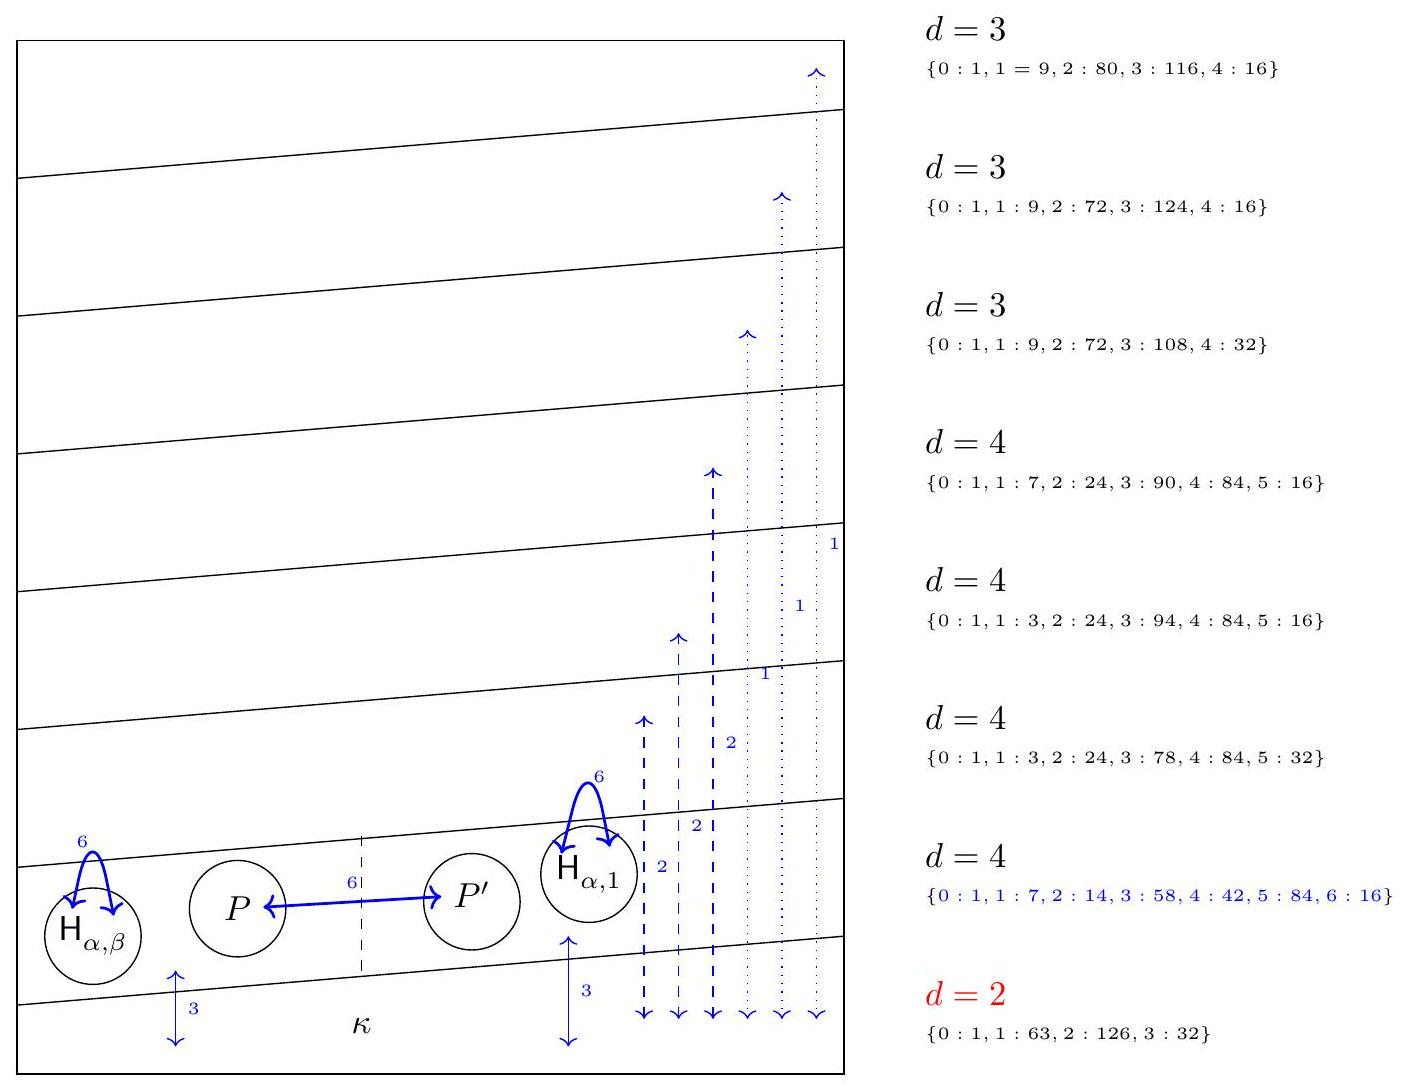
\includegraphics[alt={},max width=\textwidth]{d49c1314-1fbe-4a5e-99d5-489266dc6d5e-29_1091_1408_438_322}
\captionsetup{labelformat=empty}
\caption{Figure 1: The overall structure of the CCZ-class of the Kim mapping $\kappa$. The 8 parts correspond to one EA-class or a set of EA-classes characterized by a particular thickness spectrum. The circles correspond to the four affine equivalence classes of permutations, and arrows correspond to $t$-twists.}
\end{center}
\end{figure}

\begin{table}[h]
\begin{center}
\begin{tabular}{|l|l|}
\hline
$i$ & Univariate representation \\
\hline
1 & $x^{3}$ \\
\hline
2 & $x^{3}+\alpha^{11} x^{6}+\alpha x^{9}$ \\
\hline
3 & $\alpha x^{5}+x^{9}+\alpha^{4} x^{17}+\alpha x^{18}+\alpha^{4} x^{20}+\alpha x^{24}+\alpha^{4} x^{34}+\alpha x^{40}$ \\
\hline
4 & $\alpha^{7} x^{3}+x^{5}+\alpha^{3} x^{9}+\alpha^{4} x^{10}+x^{17}+\alpha^{6} x^{18}$ \\
\hline
5 & $x^{3}+x^{10}+\alpha x^{24}$ \\
\hline
6 & $x^{3}+\alpha^{17} x^{17}+\alpha^{17} x^{18}+\alpha^{17} x^{20}+\alpha^{17} x^{24}$ \\
\hline
7 & $x^{3}+\alpha^{11} x^{5}+\alpha^{13} x^{9}+x^{17}+\alpha^{11} x^{33}+x^{48}$ \\
\hline
8 & $\alpha^{25} x^{5}+x^{9}+\alpha^{38} x^{12}+\alpha^{25} x^{18}+\alpha^{25} x^{36}$ \\
\hline
9 & $\alpha^{40} x^{5}+\alpha^{10} x^{6}+\alpha^{62} x^{20}+\alpha^{35} x^{33}+\alpha^{15} x^{34}+\alpha^{29} x^{48}$ \\
\hline
10 & $\alpha^{34} x^{6}+\alpha^{52} x^{9}+\alpha^{48} x^{12}+\alpha^{6} x^{20}+\alpha^{9} x^{33}+\alpha^{23} x^{34}+\alpha^{25} x^{40}$ \\
\hline
11 & $x^{9}+\alpha^{4} x^{10}+\alpha^{9} x^{12}+\alpha^{4} x^{18}+\alpha^{9} x^{20}+\alpha^{9} x^{40}$ \\
\hline
12 & $\alpha^{52} x^{3}+\alpha^{47} x^{5}+\alpha x^{6}+\alpha^{9} x^{9}+\alpha^{44} x^{12}+\alpha^{47} x^{33}+\alpha^{10} x^{34}+\alpha^{33} x^{40}$ \\
\hline
13 & $\alpha x^{6}+x^{9}+\alpha x^{10}+\alpha^{4} x^{17}+\alpha x^{24}+\alpha x^{33}$ \\
\hline
\end{tabular}
\captionsetup{labelformat=empty}
\caption{Table 6: The Banff list of quadratic APN functions operating on 6 bits. The element $\alpha$ is a root of $x^{6}+x^{4}+x^{3}+x+1$.}
\end{center}
\end{table}

Interestingly, all ortho-derivatives have the trivial thickness spectrum (i.e. $\{0: 1\}$ ), except for

\begin{table}[h]
\begin{center}
\begin{tabular}{|l|l|l|l|l|l|l|l|}
\hline
\multirow[t]{2}{*}{$i$} & \multirow{2}{*}{Thickness Spectrum} & \multirow{2}{*}{Linearity} & \multicolumn{2}{|c|}{rank} & \multicolumn{2}{|c|}{\# EA} & \multirow{2}{*}{Diff. Spec. of $\pi_{F}$} \\
\hline
 &  &  & г & $\Delta$ & min & max &  \\
\hline
1 & \{0:1, 1: 63, 2:126\} & 16 & 1102 & 94 & 3 & 190 & \{0:2205,2:1764,8:63\} \\
\hline
2 & \{0:1, 1:63, $2: 126$ \} & 16 & 1146 & 94 & 3 & 190 & \{0:2583,2:1008,4:378,8:63\} \\
\hline
3 & \{0:1,1:63,2:30\} & 16 & 1158 & 96 & 4 & 94 & \{0:2454,2:1176,4:370,6:30,10:2\} \\
\hline
4 & \{0:1, 1: 63, $2: 42$ \} & 16 & 1166 & 94 & 5 & 106 & \{0:2338, $2: 1428,4: 210,6: 56\}$ \\
\hline
5 & \{0:1, 1: 63, $2: 126,3: 32\}$ & 16 & 1166 & 96 & 8+1 & 222 & \{0:2373,2:1428,4:168,8:63\} \\
\hline
6 & \{0:1, 1: 63, $2: 54$ \} & 16 & 1168 & 96 & 9 & 118 & \{0:2442,2:1229,4:303,6:51,8:7\} \\
\hline
7 & \{0:1,1:63,2:30\} & 32 & 1170 & 96 & 6 & 94 & \{0:2401,2:1371,4:195,6:50,14:15\} \\
\hline
8 & \{0:1, 1: 63, $2: 42$ \} & 16 & 1170 & 96 & 8 & 106 & \{0:2426,2:1255,4:297,6:49,8:5\} \\
\hline
9 & \{0:1,1:63,2:54\} & 16 & 1170 & 96 & 9 & 118 & \{0:2439,2:1235,4:297,6:57,8:4\} \\
\hline
10 & \{0:1, 1: 63, $2: 54\}$ & 16 & 1170 & 96 & 9 & 118 & \{0:2422,2:1271,4:279,6:53,8:7\} \\
\hline
11 & \{0:1, 1: 63, $2: 42,3: 8\}$ & 16 & 1172 & 96 & 20 & 114 & \{0:2385,2:1339,4:258,6:45,8:2,12:3\} \\
\hline
12 & \{0:1, 1:63, 2:54, 3:8\} & 16 & 1172 & 96 & 20 & 126 & \{0:2404,2:1307,4:261,6:53,8:7\} \\
\hline
13 & \{0:1, 1: 63, $2: 42$ \} & 16 & 1174 & 96 & 9 & 106 & \{0:2414,2:1271,4:303,6:37,8:7\} \\
\hline
\end{tabular}
\captionsetup{labelformat=empty}
\caption{Table 7: Several CCZ-class invariants for the functions in the Banff list and bounds on the number of EA classes in their CCZ-classes.}
\end{center}
\end{table}

the cube mapping and for the Kim mapping. Their thickness spectra are given by:

$$
\begin{aligned}
\text { thickness spectrum of } \pi_{x^{3}} & =\{0: 1,3: 9,6: 54\} \\
\text { thickness spectrum of } \pi_{\kappa} & =\{0: 1,6: 5\},
\end{aligned}
$$

implying that both are EA-equivalent to permutations.

\subsection*{4.5 8-bit Quadratic APN functions}
As Dillon et al. derived their APN permutation on 6 variables from a quadratic APN function, there have been attempts to reproduce this general approach by finding ways to generate large numbers of quadratic APN functions on an even number of variables, and then checking if they are in fact CCZ-equivalent to a permutation. While none of the obtained functions is CCZ-equivalent to a permutation, more than 20,000 distinct 8 -bit quadratic APN functions have been exhibited, the first 8,000 having been obtained using the QAM [YWL14], and the next 12,000 through an optimized guess-and-determine approach focusing on functions with internal symmetries BL21, BL20.

Combining both lists gave us 21,102 distinct quadratic APN functions. It turns out that all of these functions can be put into distinct buckets in a few minutes using the extended Walsh spectrum and differential spectrum of their ortho-derivative as a distinguisher. The fact that these functions are thus in distinct CCZ-equivalence classe ${ }^{8}$ is not a new result ${ }^{9}$ but the speed of our method is noteworthy (see also Kal20). It has a low memory complexity, and handles the 21102 8 -bit functions under investigation in about 70 seconds on a desktop computer 10 The second best invariant for this purpose is undoubtedly the $\Sigma^{4}$-multiplicities, which takes 19367 distinct values for our functions, meaning that it has almost the same distinguishing power as the orthoderivative. The computation of the $\Sigma^{4}$-multiplicities took about 1 hour and 26 minutes on the same computer. We thus claim that our ortho-derivative-based approach is at the moment the best solution to the EA-partitioning problem in the case of quadratic APN functions. While this setting may be narrow, it is arguably one of the most interesting ones.

\footnotetext{${ }^{8}$ Recall that CCZ-equivalence and EA-equivalence coincide in the case of quadratic APN functions Yos11.\\
${ }^{9}$ In fact, the authors of BL21 used our method based on the ortho-derivative - and indeed our implementationto solve this problem.\\
${ }^{10}$ More precisely, all these experiments were run on a dell Precision 3630 with an Intel Core i5-8500 CPU at 3.00 GHz , and 32 GB of RAM.
}We can still use the other invariants to learn more about these functions. First, there are only 6 distinct extended Walsh spectra in the whole list of the 21,102 known 8 -bit quadratic APN functions:

$$
\begin{aligned}
& \{0: 16320,16: 43520,32: 5440\}, \\
& \{0: 15600,16: 44544,32: 5120,64: 16\}, \\
& \{0: 14880,16: 45568,32: 4800,64: 32\}, \\
& \{0: 14160,16: 46592,32: 4480,64: 48\}, \\
& \{0: 13440,16: 47616,32: 4160,64: 64\}, \\
& \{0: 12540,16: 48640,32: 4096,128: 4\},
\end{aligned}
$$

meaning that there are many functions with identical extended Walsh spectra but distinct thickness spectra. On the other hand, some functions have identical thickness spectra but different Walsh spectra (see the bottom of Table 8 for an example). There are $255=2^{8}-1$ different thickness spectra, a number that looks interesting in itself. Indeed, recall that there are $7=2^{3}-1$ different thickness spectra among all 6 -bit quadratic APN functions.

We can also fit all these functions into 486 different buckets with distinct extended Walsh spectrum/thickness spectrum pairs. However, the functions are not uniformly spread among said buckets, in fact only 10 of these classes account for about a third of all functions (see the first rows of Table 8). We remark that, for all these large classes, the number of spaces of thickness 2 is always a multiple of 6 , and that the 10 most common thickness spectra correspond to those having between 108 and 162 spaces of thickness 2. However, it is not necessary for $N_{2}$ to be a multiple of 6 as witnessed for example by the function with thickness spectrum such that $N_{2}=104 \equiv 2$ mod 6 (see line 11 of Table 8).

\begin{table}[h]
\begin{center}
\begin{tabular}{|l|l|l|}
\hline
Cardinality & Extended Walsh spectrum & Thickness Spectrum \\
\hline
617 & \{0:16320, 16:43520, 32:5440\} & $\{0: 1,1: 255,2: 162\}$ \\
\hline
681 & \{0:16320, $16: 43520,32: 5440\}$ & $\{0: 1,1: 255,2: 156\}$ \\
\hline
617 & $\{0: 16320,16: 43520,32: 5440\}$ & $\{0: 1,1: 255,2: 150\}$ \\
\hline
606 & \{0:16320, 16:43520, 32:5440\} & $\{0: 1,1: 255,2: 144\}$ \\
\hline
640 & \{0:16320, 16:43520, 32:5440\} & $\{0: 1,1: 255,2: 138\}$ \\
\hline
681 & \{0:16320, 16:43520, 32:5440\} & $\{0: 1,1: 255,2: 132\}$ \\
\hline
635 & $\{0: 16320,16: 43520,32: 5440\}$ & $\{0: 1,1: 255,2: 126\}$ \\
\hline
664 & \{0:16320, 16:43520, 32:5440\} & $\{0: 1,1: 255,2: 120\}$ \\
\hline
639 & \{0:16320, 16:43520, 32:5440\} & $\{0: 1,1: 255,2: 114\}$ \\
\hline
616 & \{0:16320, $16: 43520,32: 5440\}$ & $\{0: 1,1: 255,2: 108\}$ \\
\hline
1 & \{0:16320,16:43520,32:5440\} & $\{0: 1,1: 255,2: 104\}$ \\
\hline
22 & $\{0: 15600,16: 46520,32: 5440\}$ & $\{0: 1,1: 255\}$ \\
\hline
1 & $\{0: 16320,16: 43520,32: 5440\}$ & $\{0: 1,1: 255,2: 294,3: 56,4: 64\}$ \\
\hline
1 & \{0:16320, 16:43520, 32:5440\} & $\{0: 1,1: 255,2: 210,3: 56,4: 64\}$ \\
\hline
78 & \{0:15600, 16:43520, $32: 5440$ \} & \{0:1,1:255,2:194\} \\
\hline
9 & $\{0: 15600,16: 44544,32: 5120,64: 16\}$ & $\{0: 1,1: 255,2: 194\}$ \\
\hline
\end{tabular}
\captionsetup{labelformat=empty}
\caption{Table 8: The properties of some interesting classes of 8-bit quadratic APN functions.}
\end{center}
\end{table}

Focusing now on the least common spectra, we observe that 143 functions belong to classes that contain only one function. For instance, the function with the highest number of vector spaces of dimension $n$ in its Walsh zeroes (669 in total) does not share its thickness spectrum with any other APN function in the list. Only two functions have spaces of thickness 4 in their Walsh zeroes.

All functions have $N_{1}=255$, a quantity which was explained to be related to the derivatives of quadratic functions in CP19. Interestingly, there are 22 functions for which there is nothing else in the thickness spectrum. The most prominent function in this set is the cube mapping $x \mapsto x^{3}$. There is a wide variety of thickness spectra of the form $N_{0}=1, N_{1}=255, N_{2}=\ell$ as $\ell$ varies from 12 to 264 . We give the number of functions with each such thickness spectrum in Figure 2 (the Walsh spectra are not taken into account in this figure). As we can see, most functions satisfy $N_{2} \equiv 0 \bmod 6$, and the distribution of such functions seems to follow a Gaussian distribution with mean 132.06 . There are fewer functions satisfying $N_{2} \not \equiv 0 \bmod 6$, and those seem to follow their own Gaussian distribution with a different mean of 166.50.

\begin{figure}[h]
\begin{center}
  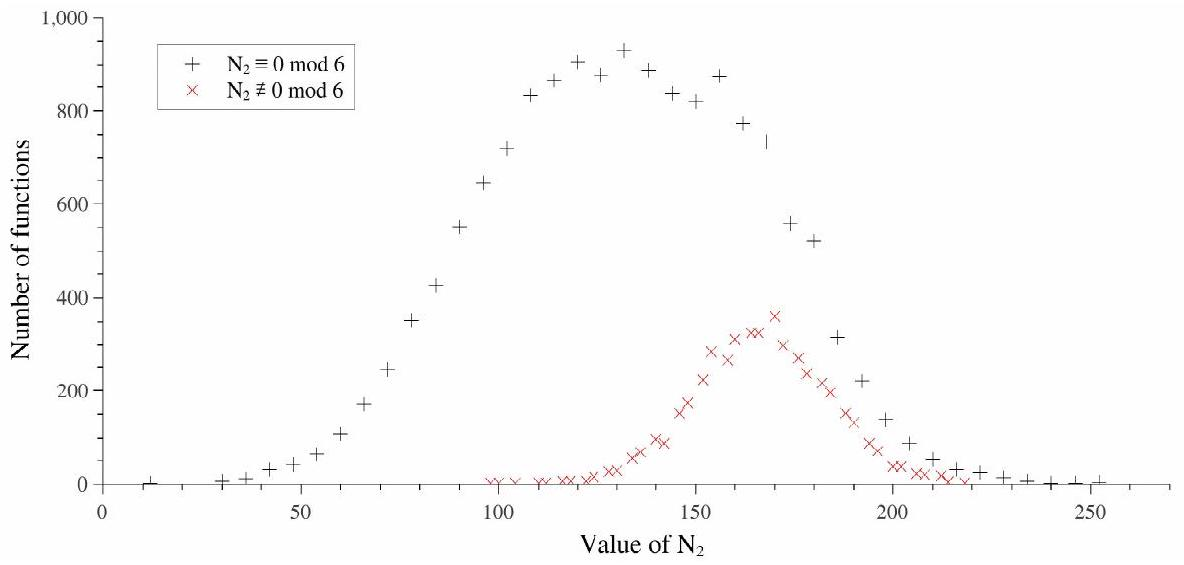
\includegraphics[alt={},max width=\textwidth]{d49c1314-1fbe-4a5e-99d5-489266dc6d5e-32_565_1184_847_438}
\captionsetup{labelformat=empty}
\caption{Figure 2: The number of known 8-bit quadratic APN functions such that the spaces in their Walsh zeroes have a maximum thickness of 2 . Different symbols are used depending on whether $N_{2} \equiv 0 \bmod 6$ or not.}
\end{center}
\end{figure}

Finally, we remark that the ortho-derivatives of all of the more than 20,000 functions we investigated have a trivial thickness spectrum, i.e. $\{0: 1\}$.

\section*{5 Conclusion}
We can efficiently solve both EA-recovery and EA-partitioning in a new set of cases, especially for quadratic APN functions that are of the most importance to researchers working on the big APN problem. In particular, our use of the ortho-derivative of quadratic APN functions for EApartitioning has already enabled us to classify the new APN functions found in BL21.

However, a general solution to both problems that could be applied in all cases, without conditions on the algebraic degree of the functions or on the form of the affine mappings involved, remains to be found.

\section*{References}
[BC10] Lilya Budaghyan and Claude Carlet. CCZ-equivalence of single and multi output boolean functions. In Post-proceedings of the 9-th International Conference on Finite Fields and Their Applications, volume 518, pages 43-54. American Mathematical Society, 2010.\\[0pt]
[BCC+ 21] Lilya Budaghyan, Marco Calderini, Claude Carlet, Robert S. Coulter, and Irene Villa. Generalized isotopic shift construction for APN functions. Des. Codes Cryptogr., 89(1):19-32, 2021.\\[0pt]
[BCHK20] Lilya Budaghyan, Claude Carlet, Tor Helleseth, and Nikolay S. Kaleyski. On the distance between APN functions. IEEE Trans. Inf. Theory, 66(9):5742-5753, 2020.\\[0pt]
[BCP06] Lilya Budaghyan, Claude Carlet, and Alexander Pott. New classes of almost bent and almost perfect nonlinear polynomials. IEEE Transactions on Information Theory, 52(3):1141-1152, 2006.\\[0pt]
[BCV20] Lilya Budaghyan, Marco Calderini, and Irene Villa. On relations between CCZ- and EA-equivalences. Cryptogr. Commun., 12(1):85-100, 2020.\\[0pt]
[BDBP03] Alex Biryukov, Christophe De Cannière, An Braeken, and Bart Preneel. A toolbox for cryptanalysis: Linear and affine equivalence algorithms. In Eli Biham, editor, EUROCRYPT 2003, volume 2656 of LNCS, pages 33-50. Springer, Heidelberg, May 2003.\\[0pt]
[BDKM09] K. A. Browning, J.F. Dillon, R.E. Kibler, and M. T. McQuistan. APN Polynomials and Related Codes. J. of Combinatorics, Information and System Sciences, 34(1-4):135-159, 2009.\\[0pt]
[BDMW10] K. A. Browning, J.F. Dillon, M. T. McQuistan, and A. J. Wolfe. An APN permutation in dimension six. In Post-proceedings of the 9-th International Conference on Finite Fields and Their Applications, volume 518, pages 33-42. American Mathematical Society, 2010.\\[0pt]
[BK12] Lilya Budaghyan and Oleksandr Kazymyrov. Verification of restricted EA-equivalence for vectorial boolean functions. In Ferruh Özbudak and Francisco RodríguezHenríquez, editors, Arithmetic of Finite Fields - WAIFI 2012, pages 108-118, Berlin, Heidelberg, 2012. Springer Berlin Heidelberg.\\[0pt]
[BL20] Christof Beierle and Gregor Leander. New Instances of Quadratic APN Functions in Dimension Eight, September 2020.\\[0pt]
[BL21] Christof Beierle and Gregor Leander. New instances of quadratic APN functions. IEEE Transactions on Information Theory, 2021.\\[0pt]
[BN15] Céline Blondeau and Kaisa Nyberg. Perfect nonlinear functions and cryptography. Finite Fields and Their Applications, 32:120-147, 2015. Special Issue : Second Decade of FFA .\\[0pt]
[BPT19] Xavier Bonnetain, Léo Perrin, and Shizhu Tian. Anomalies and vector space search: Tools for S-box analysis. In Steven D. Galbraith and Shiho Moriai, editors, ASIACRYPT 2019, Part I, volume 11921 of LNCS, pages 196-223. Springer, Heidelberg, December 2019.\\[0pt]
[BS91] Eli Biham and Adi Shamir. Differential cryptanalysis of DES-like cryptosystems. In Alfred J. Menezes and Scott A. Vanstone, editors, CRYPTO'90, volume 537 of LNCS, pages 2-21. Springer, Heidelberg, August 1991.\\[0pt]
[Cal20] Marco Calderini. On the EA-classes of known APN functions in small dimensions. Cryptogr. Commun., 12(5):821-840, 2020.\\[0pt]
[Car21] Claude Carlet. Boolean Functions for Cryptography and Coding Theory. Cambridge University Press, Cambridge, 2021.\\[0pt]
[CCZ98] Claude Carlet, Pascale Charpin, and Victor Zinoviev. Codes, bent functions and permutations suitable for DES-like cryptosystems. Designs, Codes and Cryptography, 15(2):125-156, 1998.\\[0pt]
[CDP17] Anne Canteaut, Sébastien Duval, and Léo Perrin. A generalisation of Dillon's APN permutation with the best known differential and nonlinear properties for all fields of size $2^{4 k+2}$. IEEE Transactions on Information Theory, 63(11):7575-7591, Nov 2017.\\[0pt]
[CFS14] Wieb Cannon, John amd Bosma, Claus Fieker, and Allan Steel, editors. Handbook of Magma functions. \href{https://www.math.uzh.ch/sepp/magma-2.20.4-cr/}{https://www.math.uzh.ch/sepp/magma-2.20.4-cr/}, 2.20 edition, 2014.\\[0pt]
[CP19] Anne Canteaut and Léo Perrin. On CCZ-equivalence, extended-affine equivalence, and function twisting. Finite Fields and Their Applications, 56:209-246, 2019.\\[0pt]
[Din18] Itai Dinur. An improved affine equivalence algorithm for random permutations. In Jesper Buus Nielsen and Vincent Rijmen, editors, EUROCRYPT 2018, Part I, volume 10820 of LNCS, pages 413-442. Springer, Heidelberg, April / May 2018.\\[0pt]
[EP09] Yves Edel and Alexander Pott. On the equivalence of nonlinear functions. In Bart Preneel, Stefan M. Dodunekov, Vincent Rijmen, and Svetla Nikova, editors, Enhancing Cryptographic Primitives with Techniques from Error Correcting Codes, volume 23 of NATO Science for Peace and Security Series - D: Information and Communication Security, pages 87-103. IOS Press, 2009.\\[0pt]
[Gor19] Anastasiya Gorodilova. On the differential equivalence of APN functions. Cryptogr. Commun., 11(4):793-813, 2019.\\[0pt]
[Gor20] Anastasiya Gorodilova. A note on the properties of associated boolean functions of quadratic APN functions. Prikladnaya Diskretnaya Matematika, 47, 2020.\\[0pt]
[GP21] Faruk Göloglu and Jirí Pavlu. On CCZ-inequivalence of some families of almost perfect nonlinear functions to permutations. Cryptogr. Commun., 13(3):377-391, 2021.\\[0pt]
[Jou09] Antoine Joux. Algorithmic Cryptanalysis. Chapman \& Hall/CRC, 2009.\\[0pt]
[Kal20] Nikolay Kaleyski. Deciding EA-equivalence via invariants. SETA'20. Available online: \href{https://seta-2020.org/assets/files/program/papers/paper-44.pdf.,}{https://seta-2020.org/assets/files/program/papers/paper-44.pdf.,} 2020.\\[0pt]
[Kal21a] Nikolay Kaleyski. Invariants for EA- and CCZ-equivalence of APN and AB functions. Cryptology ePrint Archive, Report 2021/300, 2021. \href{https://eprint.iacr.org/2021/300}{https://eprint.iacr.org/2021/300}.\\[0pt]
[Kal21b] Nikolay Kaleyski. Towards a deeper understanding of APN functions and related longstanding problems. PhD thesis, Bergen University, Department of Informatics, August 2021. Available online at \href{https://bora.uib.no/bora-xmlui/handle/11250/2770059}{https://bora.uib.no/bora-xmlui/handle/11250/2770059}\\[0pt]
[Kyu07] Gohar M. M. Kyureghyan. Crooked maps in $\mathbb{F}_{2^{n}}$. Finite Fields and Their Applications, 13(3):713-726, 2007.\\[0pt]
[Leo95] Jeffrey S. Leon. Partitions, refinements, and permutation group computation. In Larry Finkelstein and William M. Kantor, editors, Groups and Computation - Proceedings of a DIMACS Workshop, volume 28 of DIMACS Series in Discrete Mathematics and Theoretical Computer Science, pages 123-158. DIMACS/AMS, 1995.\\[0pt]
[Mat94] Mitsuru Matsui. Linear cryptanalysis method for DES cipher. In Tor Helleseth, editor, EUROCRYPT'93, volume 765 of LNCS, pages 386-397. Springer, Heidelberg, May 1994.\\[0pt]
[MS77] F. J. MacWilliams and N. J. A. Sloane. The Theory of Error Correcting Codes. North Holland, 1977.\\[0pt]
[NK93] Kaisa Nyberg and Lars R. Knudsen. Provable security against differential cryptanalysis (rump session). In Ernest F. Brickell, editor, CRYPTO'92, volume 740 of LNCS, pages 566-574. Springer, Heidelberg, August 1993.\\[0pt]
[Nyb91] Kaisa Nyberg. Perfect nonlinear S-boxes. In Donald W. Davies, editor, EUROCRYPT'91, volume 547 of LNCS, pages 378-386. Springer, Heidelberg, April 1991.\\[0pt]
[Nyb94] Kaisa Nyberg. Differentially uniform mappings for cryptography. In Tor Helleseth, editor, EUROCRYPT'93, volume 765 of LNCS, pages 55-64. Springer, Heidelberg, May 1994.\\[0pt]
[Nyb12] Kaisa Nyberg. "provable" security against differential and linear cryptanalysis (invited talk). In Anne Canteaut, editor, FSE 2012, volume 7549 of LNCS, pages 1-8. Springer, Heidelberg, March 2012.\\[0pt]
[ÖSY14] Ferruh Özbudak, Ahmet Sinak, and Oguz Yayla. On verification of restricted extended affine equivalence of vectorial Boolean functions. In Çetin Kaya Koç, Sihem Mesnager, and Erkay Savas, editors, WAIFI 2014, volume 9061 of LNCS, pages 137-154. Springer, Heidelberg, September 2014.\\[0pt]
[PUB16] Léo Perrin, Aleksei Udovenko, and Alex Biryukov. Cryptanalysis of a theorem: Decomposing the only known solution to the big APN problem. In Matthew Robshaw and Jonathan Katz, editors, CRYPTO 2016, Part II, volume 9815 of LNCS, pages 93-122. Springer, Heidelberg, August 2016.\\[0pt]
[S ${ }^{+} 19$ ] W. A. Stein et al. SageMath, the Sage Mathematics Software System (Version 8.6), 2019. \href{http://www.sagemath.org}{http://www.sagemath.org}.\\[0pt]
[WTG13] Guobiao Weng, Yin Tan, and Guang Gong. On quadratic almost perfect nonlinear functions and their related algebraic object. In Workshop on Coding and Cryptography, WCC, 2013.\\[0pt]
[Yos11] Satoshi Yoshiara. Equivalences of quadratic APN functions. Journal of Algebraic Combinatorics, 35:461-475, September 2011.\\[0pt]
[YWL14] Yuyin Yu, Mingsheng Wang, and Yongqiang Li. A matrix approach for constructing quadratic APN functions. Designs, Codes and Cryptography, 73(2):587-600, Nov 2014.


\end{document}